\pdfminorversion=5
\newcommand{\mytitle}{Multi-Gigabit Sub-Nyquist Sampling 60 GHz Receiver}
\newcommand{\myname}{Lorenz Koestler}
\newcommand{\myterm}{Spring Term 2014}

\documentclass[11pt, a4paper, titlepage, twoside]{book}

\usepackage[nouppercase]{scrpage2} % Kopf- und Fusszeilen formatieren
\usepackage[hang,bf]{caption}
\usepackage{ifpdf}
\usepackage[pdftex]{graphicx} \message{ETHkopf} 
\usepackage{fullpage}
\usepackage[
  colorlinks=true,        % links are colored
  citecolor=black,         % color of cite links
  %pagecolor=blue,         % color of page links
  linkcolor=black,         % color of hyperref links
  menucolor=black,         % color of Acrobat Reader menu buttons
  urlcolor=black,          % color of urls \url{}
  bookmarks=true, hyperindex=true, breaklinks=true,
  baseurl={http://www.iis.ee.ethz.ch},
  pdftitle={\mytitle},
  pdfauthor={\myname},
  pdfsubject={DFT Core generator},
  pdfkeywords={FFT, DFT, OFDM, Radix}
]{hyperref}
\usepackage[
  style=long,
  acronym,
  nonumberlist,
  numberline,
  section=chapter,
  nomain
]{glossaries} 
\usepackage[english]{babel}
\usepackage{verbatim}
\usepackage{algorithm}
\usepackage{algpseudocode}      % for algorithms
\usepackage{cite}               % will become: [2], [5]--[7]  (using cite.sty)
\usepackage{amsmath}
\usepackage{amssymb}
\usepackage{pdfpages}
\usepackage{dirtree}
\usepackage{tikz}
\usepackage{pgfplots}
\usepackage[
  textsize=tiny,
  textwidth=2cm
]{todonotes}
\usepackage{subcaption}
\usepackage{trfsigns}

% Draft watermark
\usepackage{draftwatermark}

\makeglossaries
\makeindex

% references
\renewcommand{\eqref}[1]{(\ref{#1})}
\newcommand{\chapref}[1]{Chap.~\ref{#1}}
\newcommand{\secref}[1]{Sec.~\ref{#1}}
\newcommand{\figref}[1]{Fig.~\ref{#1}}
\newcommand{\tblref}[1]{Tbl.~\ref{#1}}
\newcommand{\appref}[1]{App.~\ref{#1}}

% Sets
\newcommand{\setN}{\mathcal{N}}

% misc. math stuff
\newcommand{\ba}{\begin{array}}
\newcommand{\ea}{\end{array}}
\newcommand{\Nh}{\frac{N}{2}}
   	% include standard macros

\begin{document}
\setlength{\headsep}{2ex}
\setlength{\headheight}{1.1\baselineskip}
\pagestyle{scrheadings}

% A %%%%%
\newacronym{ADC}{ADC}{Analog to Digital Converter}
\newacronym{ASIC}{ASIC}{Application-Specific Integrated Circuit}
\newacronym{AXI}{AXI}{Advanced eXtensible Interface}
\newacronym{AWG}{AWG}{Arbitrary Waveform Generator}
\newacronym{ack}{ack}{acknowledge}
% B %%%%%
\newacronym{BPSK}{BPSK}{Binary Phase-Sift Keying}
\newacronym{QPSK}{QPSK}{Quadrature Phase-Shift Keying}
% C %%%%%
\newacronym{CMOS}{CMOS}{Complementary Metal-Oxide-Semiconductor}
\newacronym{CPU}{CPU}{Central Processing Unit}
% D %%%%%
\newacronym{DDR}{DDR}{Double Data Rate}
\newacronym{DC}{DC}{Direct Current}
\newacronym{DMA}{DMA}{Direct Memory Access}
% E %%%%%    
\newacronym{ETH}{ETH}{Swiss Federal Institute of Technology}
\newacronym{EDK}{EDK}{Embedded Development Kit}
% F %%%%%
\newacronym{FFT}{FFT}{Fast Fourier Transform}
\newacronym{FPGA}{FPGA}{Field Programmable Gate Array}
\newacronym{FMC}{FMC}{FPGA Mezzanine Card}
\newacronym{FSM}{FSM}{Finite State Machine}
\newacronym{FIFO}{FIFO}{First-In, First-Out (Memory)}
% G %%%%%
% H %%%%%
% I %%%%%
\newacronym{IP}{IP}{Intellectual Property}
\newacronym{INetP}{IP}{Internet Protocol}o
\newacronym{IF}{IF}{Intermediate Frequency}
\newacronym{IO}{IO}{Input / Output}
\newacronym{IC}{IC}{Integrated Circuit}
% J %%%%%
% K %%%%%
% L %%%%%
\newacronym{LVDS}{LVDS}{Low-Voltage Differential Signaling}
\newacronym{LUT}{LUT}{Lookup Table}
\newacronym{LED}{LED}{Light-Emitting Diode}
\newacronym{LSBand}{LSB}{Lower Side Band}
\newacronym{LO}{LO}{Local Oscillator}
% M %%%%%
\newacronym{MSB}{MSB}{Most significant bit}
\newacronym{MIG}{MIG}{Memory Interface Generator}
\newacronym{MB}{MB}{Microblaze}
% N %%%%%
% O %%%%
% P %%%%
\newacronym{PCB}{PCB}{Printed Circuit Board}
\newacronym{PHY}{PHY}{Physical Layer}
\newacronym{PLL}{PLL}{Phase-Locked Loop}
% Q %%%%
\newacronym{QAM}{QAM}{Quadrature Amplitude Modulation}
% R %%%%%
\newacronym{RAM}{RAM}{Random-access Memory}
\newacronym{RF}{RF}{Radio Frequency}
\newacronym{RX}{RX}{Receiver / receive}
\newacronym{req}{req}{request}
\newacronym{RRC}{RRC}{Root-Raised-Cosine}
% S %%%%%
\newacronym{SGMII}{SGMII}{Serial Gigabit Media Independent Interface}
\newacronym{SNR}{SNR}{Signal to Noise Ratio}
% T %%%%%
\newacronym{TX}{TX}{Transmitter / transmitt}
% U %%%%%
\newacronym{USB}{USB}{Universal Serial Bus}
\newacronym{USBand}{USB}{Upper Side Band}
\newacronym{UI}{UI}{User Interface}
\newacronym{UDP}{UDP}{User Datagram Protocol}
\newacronym{UART}{UART}{Universal Asynchronous Receiver Transmitter}
% V %%%%%
% W %%%%%
% X %%%%%
% Y %%%%%
% Z %%%%%

% Add all glossary entries, even if they were not used in the text
\glsaddall

\frontmatter
\setlength{\parindent}{0pt}
\setlength{\parskip}{10pt}

\title{\mytitle}
\author{\myname}
\date{\myterm}

\begin{titlepage}
  \begin{center}

  \vspace*{-2cm}
  \begin{minipage}{\textwidth}
    
\includegraphics[width=0.6\textwidth]{ethlogo}
    \hfill
    \raggedright
    
\includegraphics[width=0.3108\textwidth]{epfl}
  \end{minipage}

  \vspace{3cm}

  \begin{flushright}
    {\LARGE Master Project}\\
    \vspace{5mm}

    \href{http://tcl.epfl.ch}{Telecommunication Circuits Laboratory, EPFL}


    \vspace{1.5cm} {\LARGE \bfseries \mytitle}
    \rule{\textwidth}{0.8mm}

    \vspace{2cm}

    Lorenz Koestler $ < $\href{mailto:lorenz@koestler.ch}{lorenz@koestler.ch}$ > $ \\

    \vspace{4cm}

    \myterm

    \vspace{2cm}
    Advisors: \\
    Nicholas Preyss $ < $\href{mailto:nicholas.preyss@epfl.ch}{nicholas.preyss@epfl.ch}$ > $ \\
    Prof. Andreas Burg $ < $\href{mailto:andreas.burg@epfl.ch}{andreas.burg@epfl.ch}$ > $ \\
    Dr. Norbert Felber $ < $\href{mailto:felber@iis.ee.ethz.ch}{felber@iis.ee.ethz.ch}$ > $ \\

  \end{flushright}
\end{center}
\newpage

\end{titlepage}

\chapter*{Abstract}
The \gls{DFT} processor is a key component in
\gls{OFDM} communication systems
and often needs to support different input sample sizes.
To reduce the development effort when experimenting with new mobile standards,
a \gls{FFT} Core Generator was implemented which can generate a \gls{FFT} Core for
a specific application.
Even tough our core generator is focused on \gls{OFDM},
it can also be used for many different applications.
It was designed to achieve a reasonable throughput and latency
on the smallest area possible while being configurable in terms of
\gls{FFT} point sizes and word widths.

% LocalWords:  FFT OFDM

\chapter*{Acknowledgments}
%\addcontentsline{toc}{chapter}{Acknowledgments}
My special thank goes to my supervisors Harald Kr\" oll and Sandro Belfanti for their support.
They helped me finding a very interesting topic, pointed me to the right direction during the
thesis and most importantly helped me when I was stuck.
I would also like to thank Frank G\" urkaynak and Christian Benkeser for the very helpful discussions.
I am very grateful to the \gls{IIS} at \gls{ETH} Zurich giving me the opportunity to write this thesis and for their IT support.


\tableofcontents

\listoftodos

\todo{check placement and size of all figures}
\todo{spell checking all paragraphs}
\todo{check capital / non capital words in all titels}
\todo{appendix: tables missing?}

\mainmatter

\chapter{Introduction}
\label{ch:introduction}

\section{Importance of continuous Development in
  Mobile Communication Technologies}

Mobile communication systems became so ubiquitous that most of our daily
use of information technology simply would not work without them.
In many first world countries, one has to almost search for places without
mobile cell network coverage and in third world countries the availability of
mobile communication is often better then the one of fresh water. \\

Because of their high availability, computer networks became so closely
incorporated in many applications, that the user experience of using those
application highly depends on a low latency and high bandwidth link
to a server providing data or even doing the actual task.
Therefor it is of essential importance, that
the performance of computer networks continuous \cite{web_content_delivery}
to grow exponentially at least as fast as other key factors like
\gls{CPU} speeds and memory capacities. \\

\acrshort{CMOS} technology and thereby digital signal processing capabilities
develops according to Moore's Law, while this is very unclear for analog
circuits in near future as stated in \cite{belgium}.
Therefor a trend to move processing steps from analog to digital
domain exists. \\

\section{Role of 60 GHz}
Since it won't be possible to increase the throughput of digital communication
systems forever by improving the \gls{SNR} as well as coding, channel allocation
and modulation schemes, the only way will be to increase the channel bandwidth.
While \gls{VHF} and \gls{UHF} bands are heavily used by many different
users and because implementation constraints require the channel
bandwidth to be small compared to the absolute carrier frequency,
the only way will be to use higher frequency bands. \\

Therefor this work experiments with the possibilities of the 60 GHz
\gls{ISM} band where the available setup allows for bandwidth of up to
1.8 GHz and therefor data rates up to 7.2 Gbit/s. \\

Such high data rates allow for new applications which simply were not possible
using existing wireless standards. Network storage devices can be accessed
at close distance with their full hard disk speed to provide fast file
up- and downloads. \gls{HD} video can be streamed lossless and uncompressed
over the air possibly replacing existing cable connections to video
projectors and monitors. \\

60 GHz confronts engineers with many new design constraints though. The very
high free-space path loss requires for advanced beam forming methods
for distances above a few meters.
This is not only possible using huge scale parabolic
antennas as it is done for satellite networks for decades, but can also
be done in a much more dynamic way by means of antenna arrays.
The very small wave length allows to integrate these arrays
directly on an \gls{IC}. \\

On the other hand, the high attenuation allows to reuse the same channel
in a relatively close cell. \\

While the object sizes and distances in an indoor environment stay the same,
the symbol rates on 60 GHz get much higher. Therefor the resulting
delay spread is wider and correct channel estimation and correction
gains in complexity.  \\

\section{This Thesis}
In order to analyze the different receiver designs,
to get measurements of channel characteristics,
to quantify phase noise figures and finally to find
performance limiting impairments on 60 GHz communication
systems, a versatile communication system was needed. \\

Therefor different receiver architectures were analyzed as described in
\chapref{chap:rx}. A communication system including mod- and demodulation,
pulse shaping, time and frequency synchronization as well as channel and phase noise
estimation and correction was implemented in software as described in
\chapref{chap:sys}.
\chapref{chap:fpga} describes the \gls{FPGA} design, which was developed
to interface a 3.6 GS/s \gls{ADC},
store it's data in real time, provide a fast download interface and thereby
to allow reproduction of simulation results on real hardware.
All the used \gls{RF} components were measured using a state of the art
vector network analyzer as noted in \chapref{chap:comp}.
Finally \chapref{chap:res_450} contains information
about the exact test setup and the achieved performance of the system. \\

%%  LocalWords:  interferer rx CMOS SNR Gbit HD lossless IC sys fpga
%%  LocalWords:  FPGA Moore's

\chapter{Selection of Receiver Architecture}
\label{chap:rx}

A wide variety of different receiver designs exists each with it's advantages
and drawbacks. To come up with an optimal design, different receiver designs
were investigated using theoretical considerations. Some were simulated to
get an even deeper understanding.
Thereby the focal point was on architectures we could
build in hardware using the Sivers IMA 58-63 GHz converter described in
\secref{sec:comp_sivers}. \\

In the following chapters the terms \gls{TX} \gls{USBand} and \gls{TX}
\gls{LSBand} refer to the fact that the up-mixer used for transmitting
produces two signals at $f_{\text{TX LO}} \pm f_{\text{TX IF}}$ where
$f_{\text{TX LO}}$ is the frequency of the transmitter's \gls{LO}
used by the mixer mixing up to \gls{RF}. $f_{\text{TX IF}}$ is the central
frequency of the transmitters \gls{IF} signal. During all experiments
\gls{TX} \gls{USBand} was considered the desired signal and \gls{TX}
\gls{LSBand} a residual signal. \\

Analogous \gls{RX} \gls{USBand} and \gls{RX} \gls{LSBand} refer to
the down-mixer converting energy from $f_{\text{RX LO}} \pm f_{\text{RX IF}}$
to the same receiver \gls{IF} $f_{\text{RX IF}}$. \\

\section{Transmitter Architecture}
During this report always the same transmitter architecture was used.
It consists of a two channel \gls{DAC} generating the real and imaginary
part of an analytic signal width a bandwidth $B = 1.8 \text{GHz}$
on an \gls{IF} $f_{\text{TX IF}}$. \\

This two signals are than up-converter to
\gls{RF} and a $90^\circ$ coupler is used to suppress the \gls{LSBand}
as good as possible as described in \secref{sec:rx_rf_1}.
Therefor the \gls{USBand} considered the desired signal and the
residual \gls{LSBand} an interferer. \\

It was measured that in our setup the \gls{TX} \gls{LO} leakage
to the output \gls{RF} signal has similar power than the desired
signal it self. Therefor this leakage has to be considered.
By choosing $f_{\text{TX IF}} = f_{\text{c}} - f_{\text{TX LO}}$ accordingly,
this strong signal can be placed such that it is well suppress by the channel
filter. \\

Even though this would solve the problem of the the suppression of the
undesired \gls{TX} \gls{LO} leakage, in all receivers
$f_{\text{TX LO}}$ and $f_{\text{RX LO}}$ were chosen differently.
This was done to make sure that the residual \gls{TX} \gls{LSBand}
signal does not align with the desired \gls{TX} \gls{USBand} after
down-mixing. A perfect alignment could result in an even better
\gls{SNR} due to the fact that additional signal energy is transmitted
alongside the desired \gls{TX} \gls{USBand} signal. \\

\section{RF Architecture}
When building a receiver, one faces the problem of isolating the channel of
interest from all others signals received by the antenna. Therefor
two ways of building channel selection filters are discussed in the following
chapters. \\

All receivers have a band filter directly after the antenna simply by the
fact that all components (antenna, amplifiers, mixers etc.) have a frequency
selectivity which is often optimized only for the band of interest.
An additional band filter might be added to minimize the total power supplied
to the \gls{LNA} which has the main influence of the total noise figure of
the receiver. \\

Inside this band there are typically multiple channels with a carrier frequency
$f_c$ and a bandwidth $B$. \\

Since it is hard to build adjustable filters on \gls{RF} to select one specific
channel, this selection is typically done on an \gls{IF}. In our case of a
carrier frequency of $f_c \approx 60 \text{GHz}$ this \gls{IF} $f_{\text{IF}}$
is always lower than the carrier frequency $f_c$ due to component restrictions. \\

\subsection{Image Rejection using High Intermediate Frequency}
\label{sec:rx_rf_0}
First we look at the architecture shown in \figref{fig:rx_rf_0_bd} where
the mixer uses a \gls{LO} at $f_{\text{RX LO}}$ to mix the signal $s(t)$
centered around $f_{c}$ to an \gls{IF} signal $i(t)$ at
$f_{\text{RX IF}} = f_{c} - f_{\text{RX LO}}$ as shown in \figref{fig:rx_rf_0_freq_s}
and \figref{fig:rx_rf_0_freq_i}. \\

The two signals $\pm (f_{c} + f_{\text{RX LO}})$ are not relevant since their
frequency is above 100 GHz and well beyond what the mixer output can drive. \\

$f_{\text{RX IF}}$ has to be high enough such that the undesired
\gls{RX} \gls{LSBand} signal at $-f_{\text{c}} + f_{\text{RX LO}}$
lies outside the band filter and does not convolve with the desired
\gls{RX} \gls{USBand} signal. This leads to a lower bound
$f_{\text{RX IF}} \geq B$ for the \gls{RX} \gls{IF} frequency
\footnote{%
  In fact $f_{\text{RX IF}} \geq \frac{B}{2}$
  is sufficient if later stages of the receiver can switch
  between \gls{USBand} and \gls{LSBand} reception.}. \\

A fixed channel filter is than used to suppress neighbouring channels
including the \gls{TX} \gls{LO} leakage which was also mixed down. \\

\begin{figure}[h!]
  \centering
  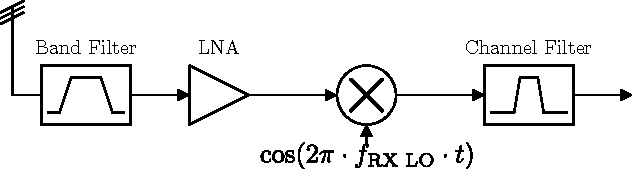
\includegraphics[width=\textwidth]{figures/rx_rf_0_bd}
  \caption{Block Diagram of Image Rejection using high \gls{IF}}
  \label{fig:rx_rf_0_bd}
\end{figure}

\begin{figure}[h!]
  \centering
  \begin{subfigure}{0.45\textwidth}
    \centering
    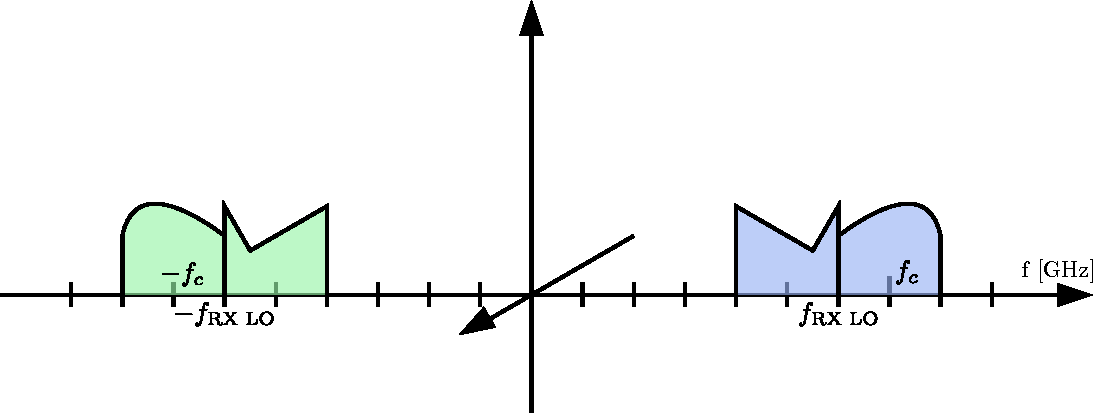
\includegraphics[width=\textwidth]{figures/rx_rf_0_freq_s}
    \caption{$s(t)$}
    \label{fig:rx_rf_0_freq_s}
  \end{subfigure}
  ~
  \begin{subfigure}{0.45\textwidth}
    \centering
    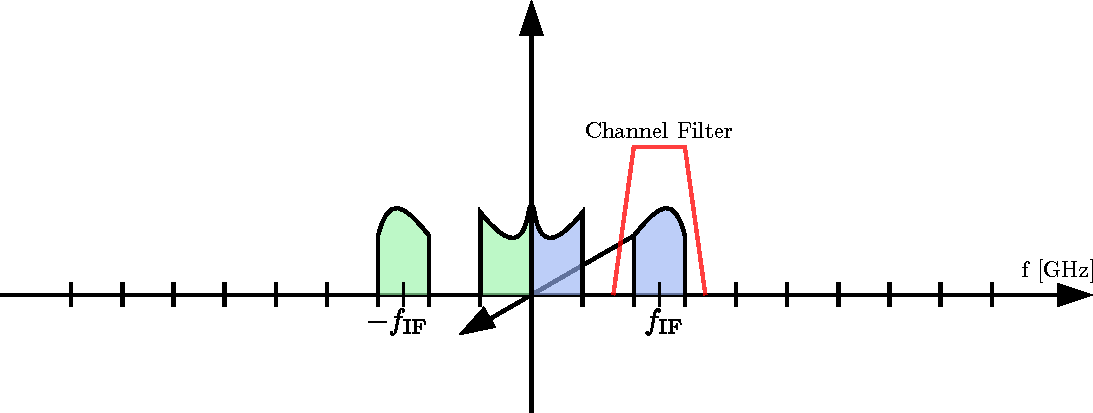
\includegraphics[width=\textwidth]{figures/rx_rf_0_freq_i}
    \caption{$i(t)$}
    \label{fig:rx_rf_0_freq_i}
  \end{subfigure}
  \caption{Image Rejection using High Intermediate Frequency}
  \label{fig:rx_rf_0_freq}
\end{figure}

\subsection{Image Rejection using $90^\circ$ Couplers}
\label{sec:rx_rf_1}
The use of a high \gls{IF} as described in the last section might
by very favorable for short wave receivers where the band filters
are very narrow (a few MHz) the \gls{IF} can be a few MHz.
For 60 GHz applications where band filters are approximately 5GHz wide,
\gls{IF} of a few GHz are required.
Therefor a more suitable way is described in this section. \\

The suppression of the undesired \gls{RX} \gls{LSBand} signal can also be done
using a $90^\circ$ couplers as described in \secref{sec:comp_90deg}: \\

Let us assume we have the real \gls{RF} signal $s(t)$ shown in
\figref{fig:rx_rf_1_freq_s}.
The blue round signal centered around the carrier frequency $+f_c$ is our
desired signal laying in the \gls{USBand} of the \gls{RX} mixer.
The spiky signal is a neighbouring channel laying exactly
where the \gls{LSBand} of the \gls{RX} mixer is and therefor has to
be suppressed.
Since it is a real signal, the negative frequencies consist of the mirrored,
complex conjugate signals which is painted in green. \\

By splitting it using a $90^\circ$ coupler we obtain the two signals
$s(t)$ and $\mathcal{H}^{-1}\{s(t)\}$ (drawn in \figref{fig:rx_rf_1_freq_Hs}).
$\mathcal{H}^{-1}$ denotes the negative Hilbert transform which rotates the phase
of a signal by $j$ for positive and $-j$ for negative frequencies
as shown in \figref{fig:hilbert}. \\

Next both signals are mixed by $f_{\text{RX LO}}$ resulting in two new signals
$a(t)$ and $b(t)$ as shown in \figref{fig:rx_rf_1_freq_a} and
\figref{fig:rx_rf_1_freq_b}.
The mirrors at $\pm (f_c + f_{\text{RX LO}})$ are already ignored. \\

By using a second $90^\circ$ coupler that applies the Hilbert transform
to $b(t)$ (drawn in \figref{fig:rx_rf_1_freq_Hb})
and adds $a(t)$ we end up with the real signal
$c(t) = a(t) + \mathcal{H}\{b(t)\}$
which is shown in \figref{fig:rx_rf_1_freq_c}. \\

One should note that the difference between $\mathcal{H}$ and $\mathcal{H}^{-1}$
is simply a swap of the two output plugs of a $90^\circ$ coupler since
the absolute phase reference is lost anyway. In fact both outputs are delayed
in time corresponding to negative phase rotation for positive frequencies
and a positive phase rotation for negative frequencies. \\

Finally a fixed channel selection filter can be used to at an arbitrary \gls{IF}
which is a clear advantage over the method discussed in \secref{sec:rx_rf_1}. \\

\begin{figure}[h!]
  \centering
  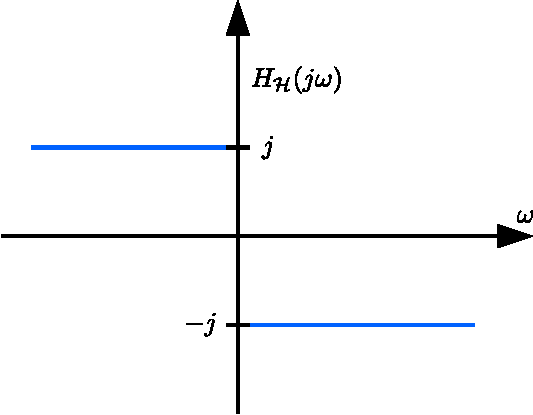
\includegraphics[width=0.3\textwidth]{figures/hilbert}
  \caption{Transfer Function of Hilbert Transform}
  \label{fig:hilbert}
\end{figure}

\begin{figure}[h!]
  \centering
  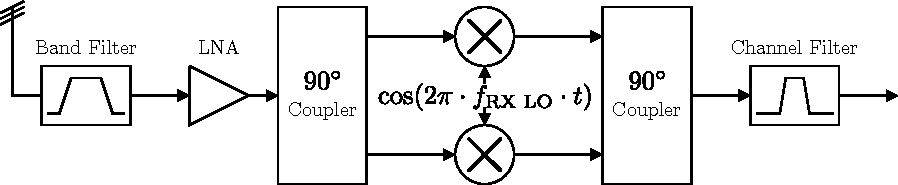
\includegraphics[width=\textwidth]{figures/rx_rf_1_bd}
  \caption{Block Diagram of Image Rejection using $90^\circ$ Couplers}
  \label{fig:rx_rf_1_bd}
\end{figure}

\begin{figure}[h!]
  \centering
  \begin{subfigure}{0.45\textwidth}
    \centering
    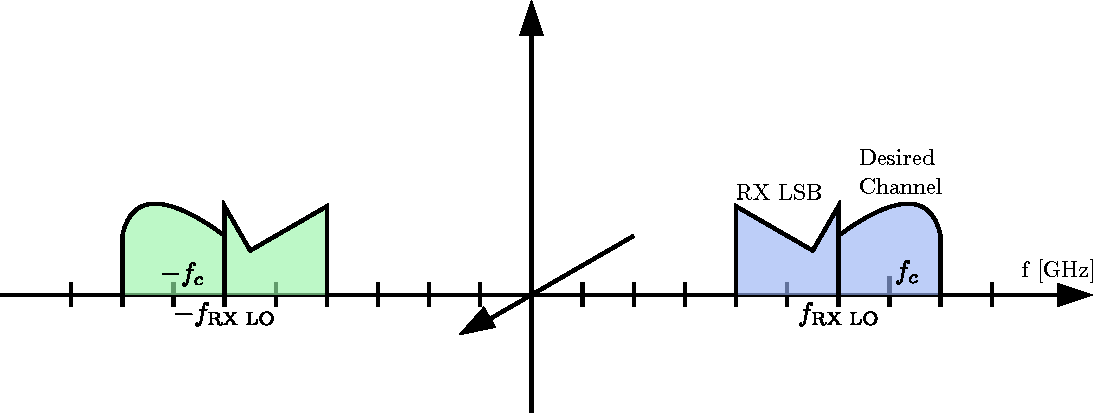
\includegraphics[width=\textwidth]{figures/rx_rf_1_freq_s}
    \caption{$s(t)$}
    \label{fig:rx_rf_1_freq_s}
  \end{subfigure}
  ~
  \begin{subfigure}{0.45\textwidth}
    \centering
    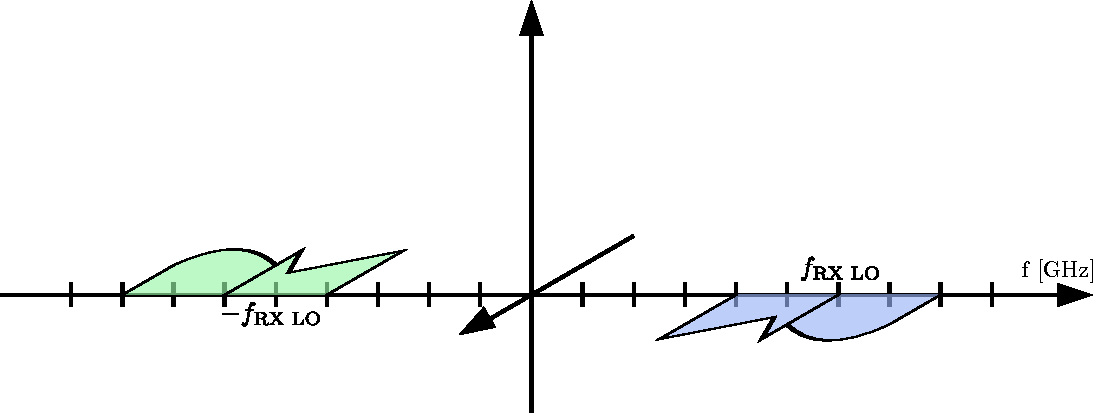
\includegraphics[width=\textwidth]{figures/rx_rf_1_freq_Hs}
    \caption{$\mathcal{H}^{-1}\{s(t)\}$}
    \label{fig:rx_rf_1_freq_Hs}
  \end{subfigure}
  \vspace{4ex} \\
  \begin{subfigure}{0.45\textwidth}
    \centering
    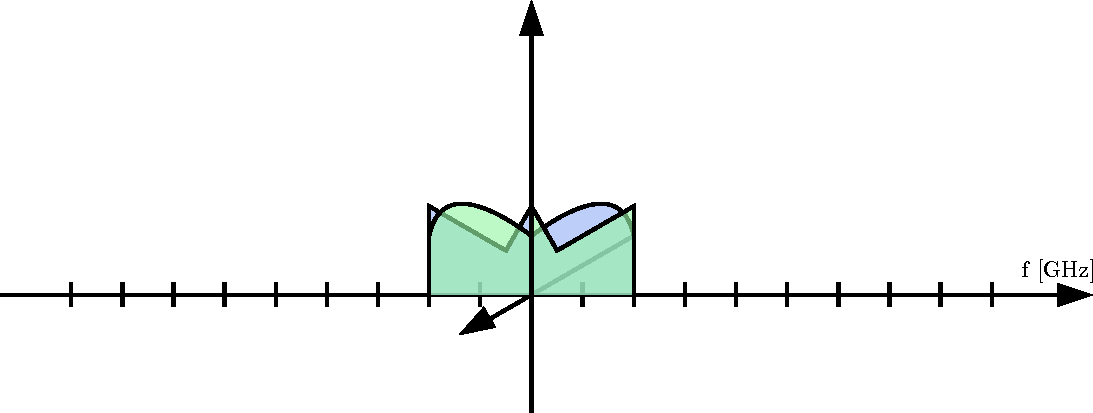
\includegraphics[width=\textwidth]{figures/rx_rf_1_freq_a}
    \caption{$a(t)$}
    \label{fig:rx_rf_1_freq_a}
  \end{subfigure}
  ~
  \begin{subfigure}{0.45\textwidth}
    \centering
    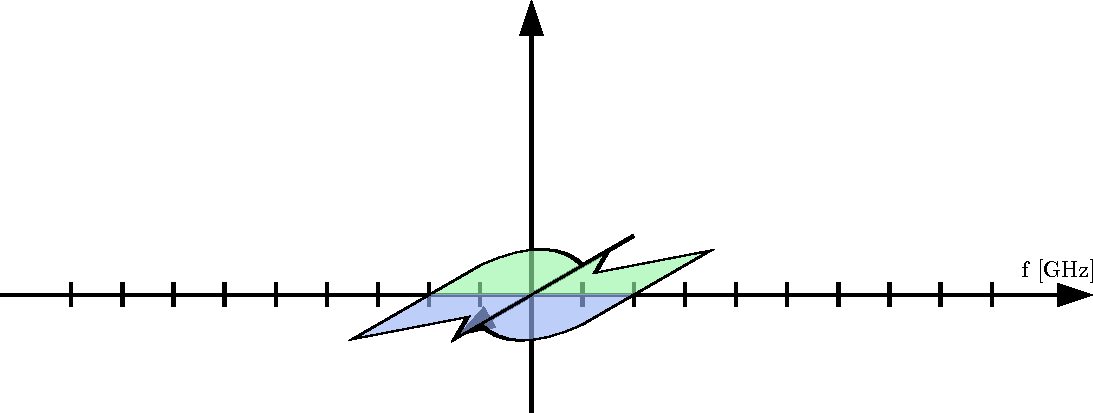
\includegraphics[width=\textwidth]{figures/rx_rf_1_freq_b}
    \caption{$b(t)$}
    \label{fig:rx_rf_1_freq_b}
  \end{subfigure}
  \vspace{4ex} \\
  \begin{subfigure}{0.45\textwidth}
    \centering
    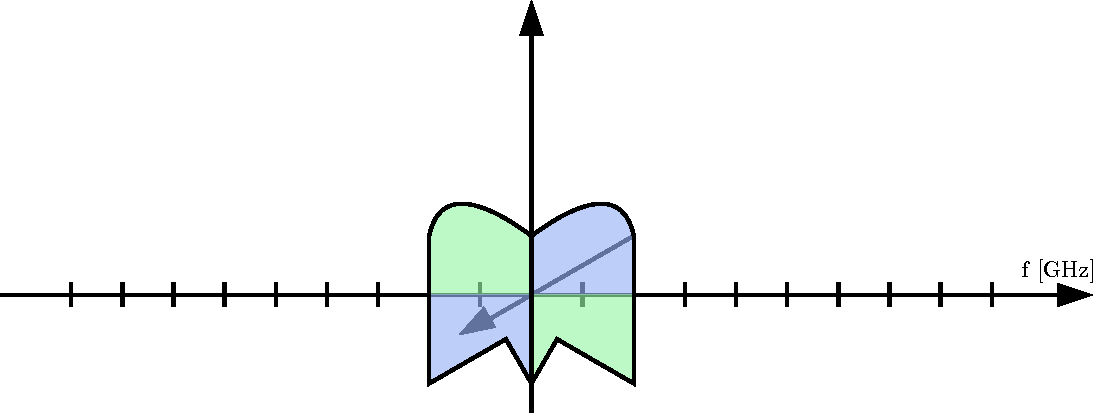
\includegraphics[width=\textwidth]{figures/rx_rf_1_freq_Hb}
    \caption{$\mathcal{H}\{b(t)\}$}
    \label{fig:rx_rf_1_freq_Hb}
  \end{subfigure}
  ~
  \begin{subfigure}{0.45\textwidth}
    \centering
    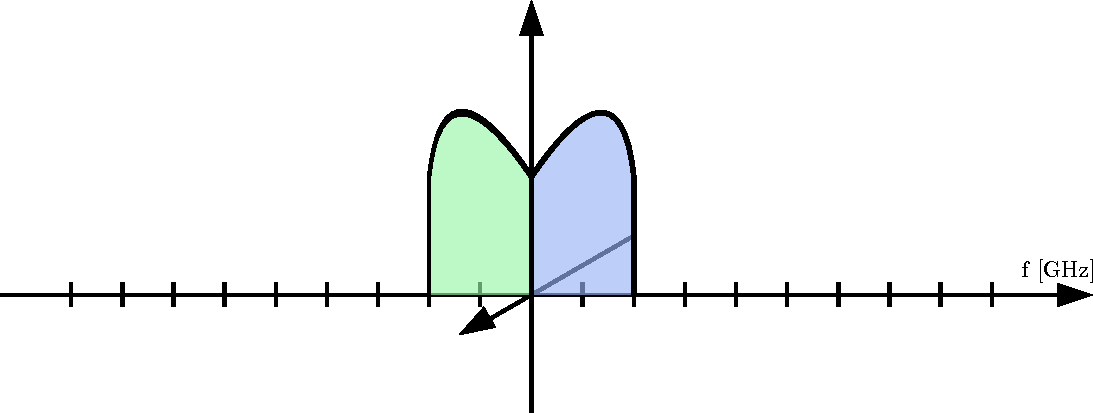
\includegraphics[width=\textwidth]{figures/rx_rf_1_freq_c}
    \caption{$c(t)$}
    \label{fig:rx_rf_1_freq_c}
  \end{subfigure}
  \caption{Image Rejection using $90^\circ$ Couplers}
  \label{fig:rx_rf_1_freq}
\end{figure}

\section{IF Architecture}
After the \gls{RF} part did the channel selection only the desired signal
is left and should be digitized.
This can be accomplished using different
mixing schemes of which three are shown in this section. \\

\subsection{Quadrature Baseband Sampling}
\label{sec:rx_adc_1}
The first \gls{IF} can be directly converted to baseband by
setting $f_{\text{LO}_2} = f_{\text{IF}}$.
Since our signal is asymmetric the baseband signal is not analytic
and therefor quadrature sampling, which uses two mixers as shown in
\figref{fig:rx_adc_1_bd}, can be used. \\

Considering a \gls{IF} signal $i(t)$ with a center frequency of $f_{\text{IF}}$
and using the transformation \eqref{eq:four_cos}
we can plot $i(t)$ mixed with $\cos(2\pi \cdot f_{\text{IF}} \cdot t)$.
See \figref{fig:rx_adc_1_freq_s}, \figref{fig:rx_adc_1_freq_cos})
and \figref{fig:rx_adc_1_freq_a}. \\

Analogous using \eqref{eq:four_sin} can be used to draw $i(t)$ mixed with
$\sin(2\pi \cdot f_{\text{IF}} \cdot t)$.
See \figref{fig:rx_adc_1_freq_sin}) and \figref{fig:rx_adc_1_freq_b}. \\

\begin{align}
  \label{eq:four_cos}
  \cos(\omega_0 \cdot t) \laplace \pi
  \left[\delta(\omega - \omega_0) + \delta(\omega + \omega_0) \right]
\end{align}

\begin{align}
  \label{eq:four_sin}
  \sin(\omega_0 \cdot t) \laplace \frac{\pi j}{2}
  \left[\delta(\omega + \omega_0) - \delta(\omega - \omega_0) \right]
\end{align}

$a(t)$ and $b(t)$ are than low pass filtered to suppress the mirror image
at $2 f_{\text{IF}}$ and sampled by a two channel \gls{ADC} running with a
sample rate $f_s \geq B$. \\

Next the analytic signal $c(t)$ is constructed without any calculations
by simply interpreting the \gls{ADC} channels as
$c(t) = b(t) + j \cdot a(t)$. To show that this works $j \cdot a(t)$
is plotted in \figref{fig:rx_adc_1_freq_ja} and
$c(t)$ in \figref{fig:rx_adc_1_freq_c}.

\begin{figure}[h!]
  \centering
  \begin{subfigure}{0.45\textwidth}
    \centering
    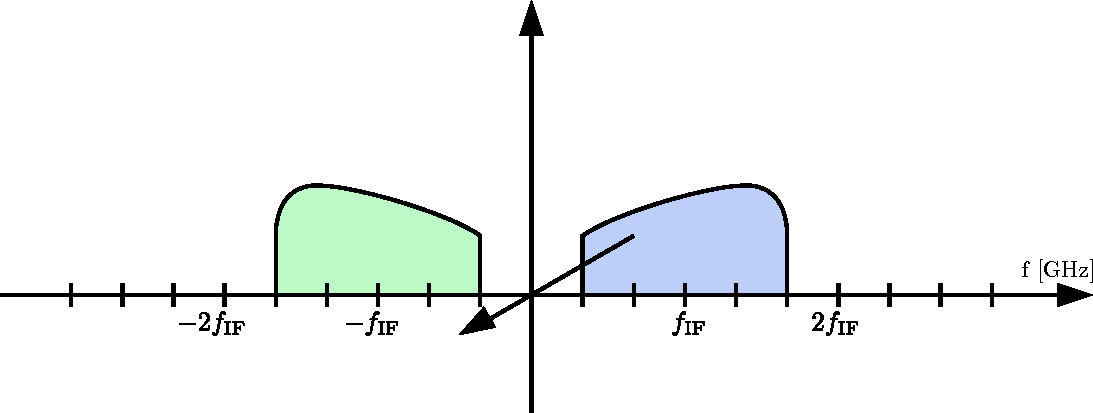
\includegraphics[width=\textwidth]{figures/rx_adc_1_freq_i}
    \caption{$i(t)$}
    \label{fig:rx_adc_1_freq_s}
  \end{subfigure}
  \vspace{4ex} \\
  \begin{subfigure}{0.45\textwidth}
    \centering
    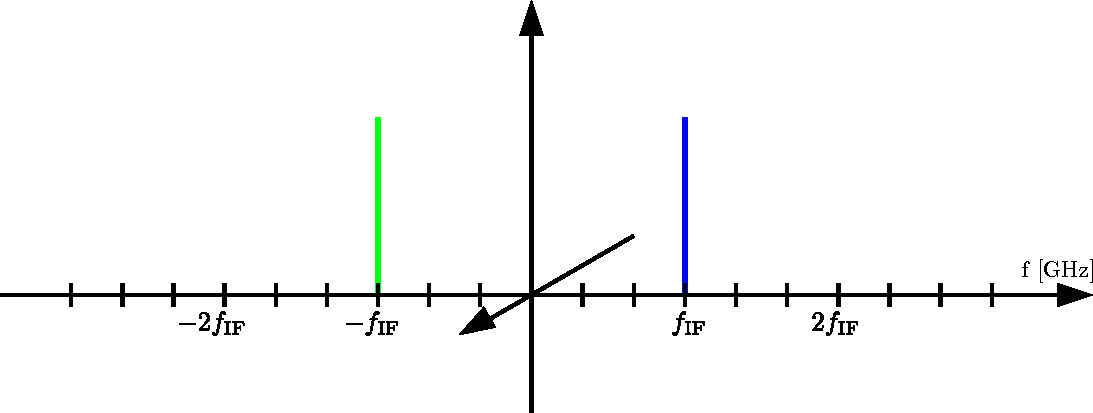
\includegraphics[width=\textwidth]{figures/rx_adc_1_freq_cos}
    \caption{$\cos(2\pi \cdot f_{\text{IF}} \cdot t)$}
    \label{fig:rx_adc_1_freq_cos}
  \end{subfigure}
  ~
  \begin{subfigure}{0.45\textwidth}
    \centering
    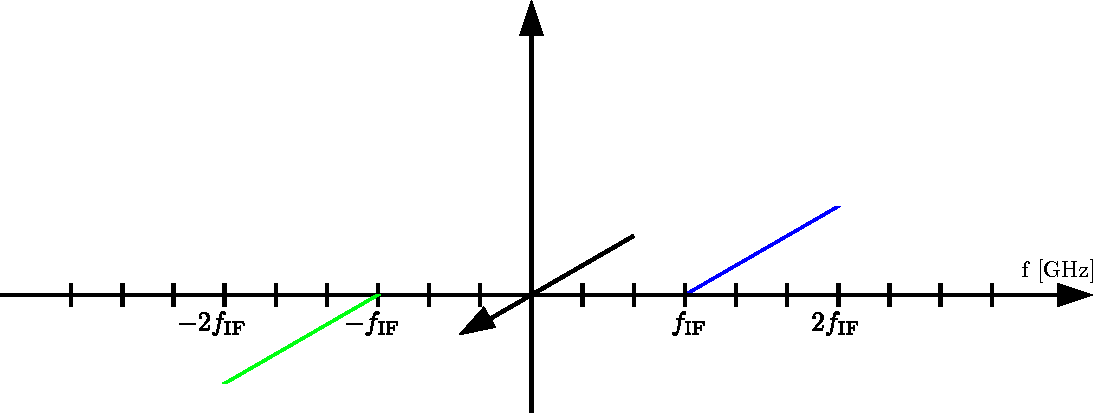
\includegraphics[width=\textwidth]{figures/rx_adc_1_freq_sin}
    \caption{$\sin(2\pi \cdot f_{\text{IF}} \cdot t)$}
    \label{fig:rx_adc_1_freq_sin}
  \end{subfigure}
  \vspace{4ex} \\
  \begin{subfigure}{0.45\textwidth}
    \centering
    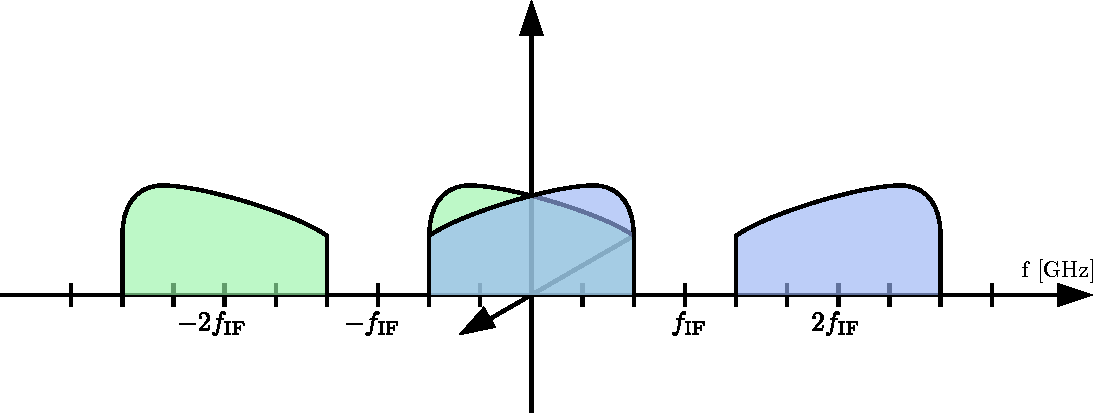
\includegraphics[width=\textwidth]{figures/rx_adc_1_freq_a}
    \caption{$a(t) = i(t) \cdot \cos(2\pi \cdot f_{\text{IF}} \cdot t)$}
    \label{fig:rx_adc_1_freq_a}
  \end{subfigure}
  ~
  \begin{subfigure}{0.45\textwidth}
    \centering
    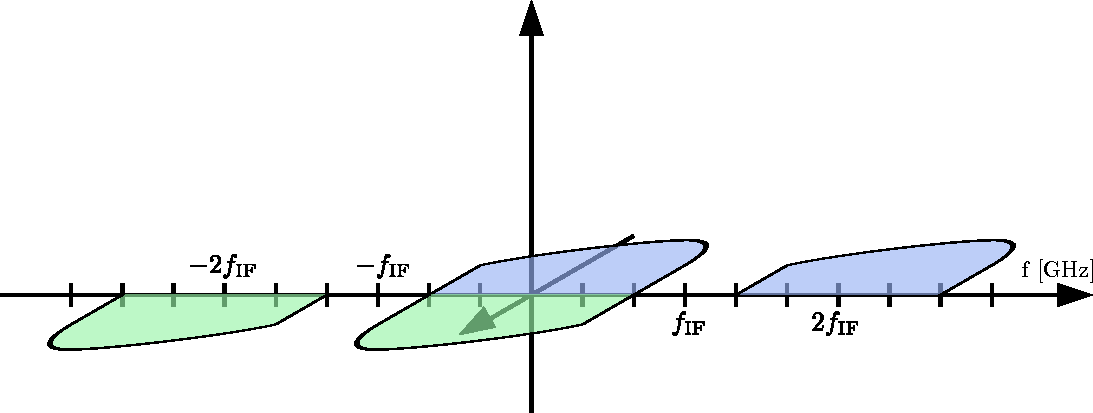
\includegraphics[width=\textwidth]{figures/rx_adc_1_freq_b}
    \caption{$b(t) = i(t) \cdot \sin(2\pi \cdot f_{\text{IF}} \cdot t)$}
    \label{fig:rx_adc_1_freq_b}
  \end{subfigure}
  \vspace{4ex} \\
  \begin{subfigure}{0.45\textwidth}
    \centering
    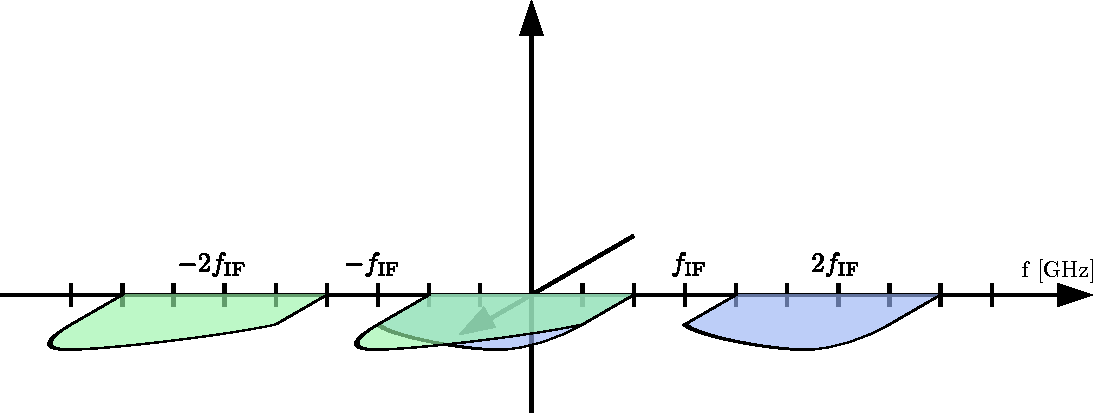
\includegraphics[width=\textwidth]{figures/rx_adc_1_freq_ja}
    \caption{$j \cdot a(t)$}
    \label{fig:rx_adc_1_freq_jb}
  \end{subfigure}
  ~
  \begin{subfigure}{0.45\textwidth}
    \centering
    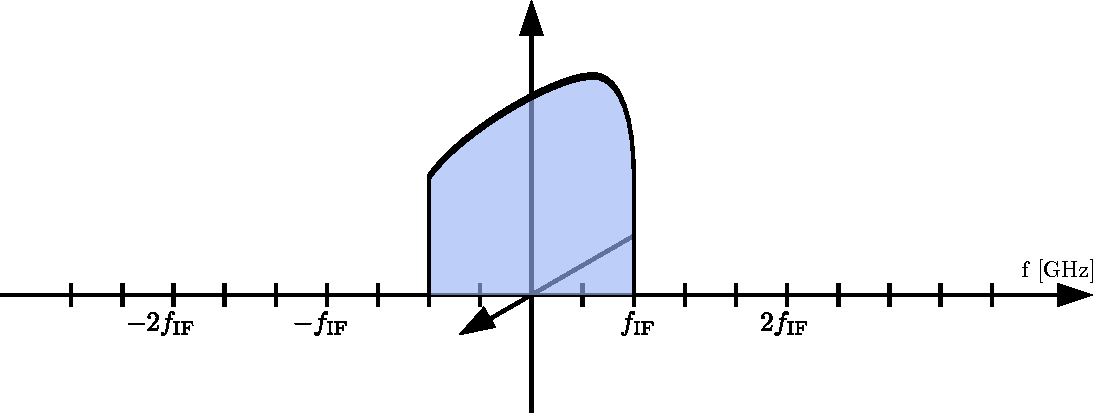
\includegraphics[width=\textwidth]{figures/rx_adc_1_freq_c}
    \caption{$c(t) = \text{LP}\{b(t)\} + j \text{LP}\{\cdot a(t)\}$}
    \label{fig:rx_adc_1_freq_c}
  \end{subfigure}
  \caption{Quadrature Baseband Mixing}
  \label{fig:rx_adc_1_freq}
\end{figure}

\begin{figure}[h!]
  \centering
  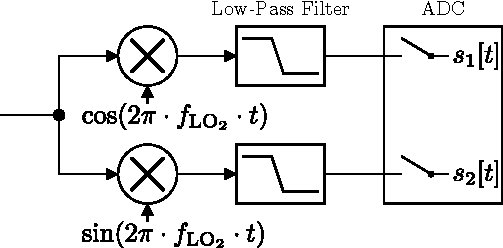
\includegraphics[width=\textwidth]{figures/rx_adc_1_bd}
  \caption{Block Diagram of Quadrature Baseband Sampling Receiver}
  \label{fig:rx_adc_1_bd}
\end{figure}

\subsection{First Nyquist-Zone Sampling}
\label{sec:rx_adc_0}
Instead of using two \gls{ADC} channels the signal can also be mixed
to the first Nyquist-zone $[0 \frac{f_s}{2}]$ and sampled by just one
channel. \\

This results in a second \gls{IF} of $f_{\text{LO}_2} = \frac{B}{2}$ where
the sampling speed $f_s$ has to be at least double the bandwidth $B$:
\[f_s \geq 2 \cdot B\]

Therefor the 1.8 GHz wide signal fully falls into the first Nyquist-zone of
a single \gls{ADC} sampling at 3.6 GHz. Again a \acrshort{DC}-block
is used in front of the \gls{ADC}. Compared to the Quadrature Baseband
Sampling Receiver only half of the signal is lost this time since
the \acrshort{DC}-block now deletes the lowest frequency part of the signal
and not the central part symmetrically around zero. Also this error
can be completely avoided by using a bandwidth $B$ slightly lower than
$\frac{f_s}{2}$. \\

\begin{figure}[h!]
  \centering
  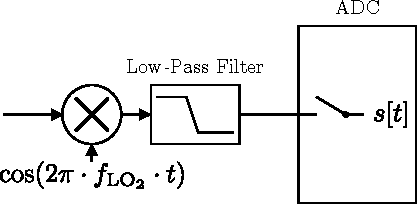
\includegraphics[width=\textwidth]{figures/rx_adc_0_bd}
  \caption{Block Diagram of First Nyquist-Zone Sampling Receiver}
  \label{fig:rx_adc_0_bd}
\end{figure}

\subsection{Quadrature Sub-Nyquist Sampling}
\label{sec:rx_adc_2}
Typically low-pass filter before the \gls{ADC} makes sure, that only
signals below $\frac{f_s}{2}$ are supplied to the sample and hold circuit
of the \gls{ADC} in order to make sure that no aliasing occurs.
$\max \frac{f_s}{2}$ is therefor the digital bandwidth of an \gls{ADC}. \\

However, an \gls{ADC} can have a bigger analog bandwidth. This means that
even faster signals are correctly captures by the sample and hold circuit
at the input of the \gls{ADC}. The frequency space between 0 and
$\frac{f_s}{2}$ is often referred to as first Nyquist-zone as shown in
\figref{fig:rx_adc_2_freq}. \\
The frequency space between $\frac{f_s}{2}$ and $f_s$ is referred to as
second Nyquist-zone. After sampling a signal, all energy captured in the
second Nyquist-zone wraps at $\frac{f_s}{2}$ and adds up with the energy
in the first Nyquist-zone. By making sure, that all significant energy
comes from only one frequency
$f \in n \cdot \frac{f_s}{2} \; \forall n \in \{1, 2, \dots\}$
no information\footnote{Except the information in which
  Nyquist-zone the signal was before sampling} is lost. \\

This trick can be combined with the Quadrature Baseband Sampling described
in \secref{sec:rx_adc_1} to capture a total bandwidth of
$B = 2 \cdot \frac{f_s}{2}$ with two channels sampling a $90^\circ$ shifted
at $f_s$ each. \\

\begin{figure}[h!]
  \centering
  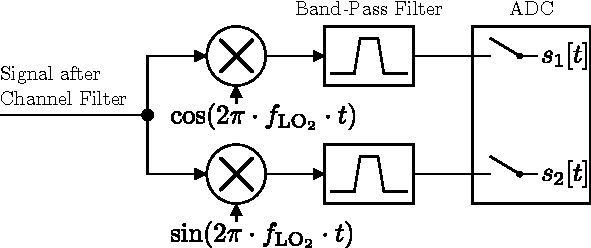
\includegraphics[width=0.7\textwidth]{figures/rx_adc_2_bd}
  \caption{Block Diagram of Quadrature Sub-Nyquist Sampling Receiver}
  \label{fig:rx_adc_2_bd}
\end{figure}

\begin{figure}[h!]
  \centering
  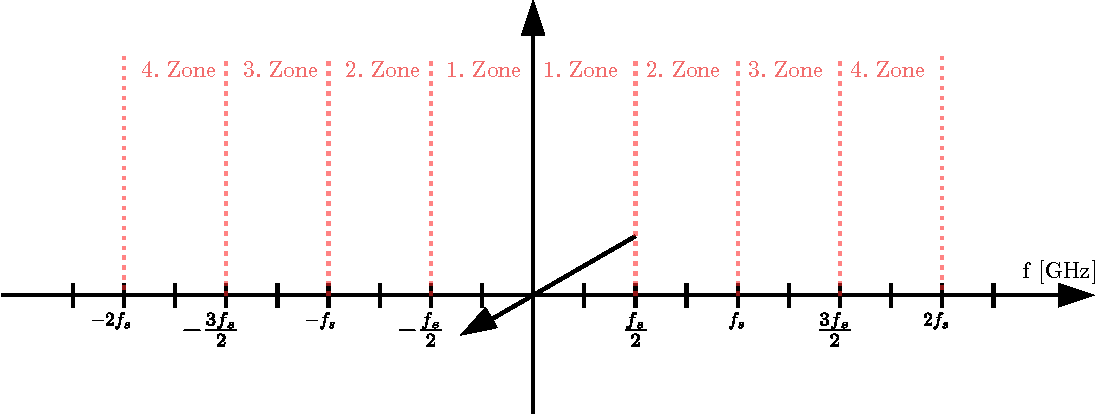
\includegraphics[width=0.7\textwidth]{figures/rx_adc_2_nyquist_zones}
  \caption{Nyquist-Zones}
  \label{fig:rx_adc_2_bd}
\end{figure}

\section{Complete Receiver Architectures}
The following sections cover three different architectures. There are example
frequencies given that are supported by the hardware available. Also their
advantages and drawbacks are discussed. \\

\subsection{Quadrature Baseband Sampling Receiver}
\label{sec:rx_0}
The Quadrature Baseband Sampling Receiver drawn in \figref{fig:rx_0_bd}
is based on the image rejection by a high enough \gls{IF} frequency as
described in \secref{sec:rx_rf_0} and than uses quadrature baseband sampling
as described in \secref{sec:rx_adc_1}.
The used frequencies are listed in \tblref{tab:rx_0} and the spectra are drawn
in \figref{fig:rx_0_freq}. \\

To do the Quadrature Baseband Sampling the
$\cos(2\pi \cdot f_{\text{LO}_2} \cdot t)$ as well as a $90^\circ$
phase shifted version $\sin(2\pi \cdot f_{\text{LO}_2} \cdot t)$ has to be
generated.
The high \gls{IF} of the receiver ($f_{\text{RX IF}} = 5.9 GHz$) requires
the \gls{LO} for the second mixing stage to run at $f_{\text{LO}_2} = 5.9 GHz$
as well which is out of the more or less linear range of the
Meca 3 dB Hybrid Coupler 705S-3.000 described in \secref{sec:comp_90deg}. \\

Self-mixing of the \gls{LO} at $f_{\text{LO}_2}$ of these mixers lead
to a \acrshort{DC}-offset which has to be blocked in order for the
\glspl{ADC} to work at full range.
Therefor all \glspl{ADC} are always used with \acrshort{DC}-blocks as described
in \secref{sec:comp_dc_block}. This high-pass filters unfortunately
not only remove \acrshort{DC} but also a small portion of the signal
resulting in some \gls{ISI}. \\

\begin{table}[h]
  \centering
  \begin{tabular}{|l|l|}
    \hline
    $f_{\text{TX IF}}$              & 1.7 GHz \\ \hline
    $f_{\text{TX LO}}$              & 59.2 GHz \\ \hline
    $f_{\text{RX LO}}$              & 55 GHz \\ \hline
    $f_{\text{RX IF}}$              & 5.9 GHz \\ \hline
    $f_{\text{LO}_2}$               & 5.9 GHz \\ \hline
    $f_c$                         & 60.9 GHz \\ \hline
    Signal Bandwidth B           & 1.8 GHz \\ \hline
    Number of \gls{ADC} channels & 2 \\ \hline
    Sample Rate $f_s$ & 1.8 GHz \\ \hline
  \end{tabular}
  \caption{Properties of Quadrature Baseband Sampling Receiver}
  \label{tab:rx_0}
\end{table}
\todo{align second col on .}

\begin{figure}[h!]
  \centering
  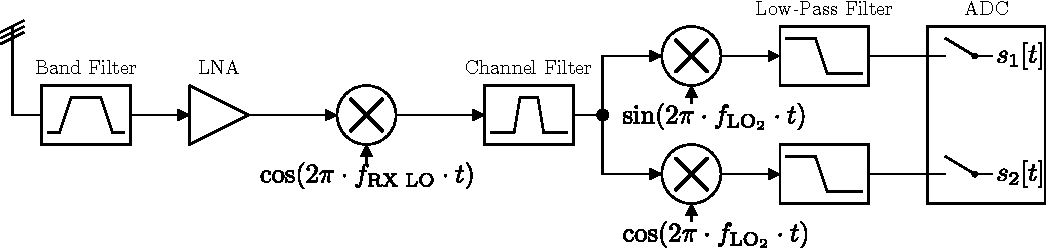
\includegraphics[width=\textwidth]{figures/rx_0_bd}
  \caption{Block Diagram of Quadrature Baseband Sampling Receiver}
  \label{fig:rx_0_bd}
\end{figure}

\begin{figure}[h!]
  \centering
  \begin{subfigure}{\textwidth}
    \centering
    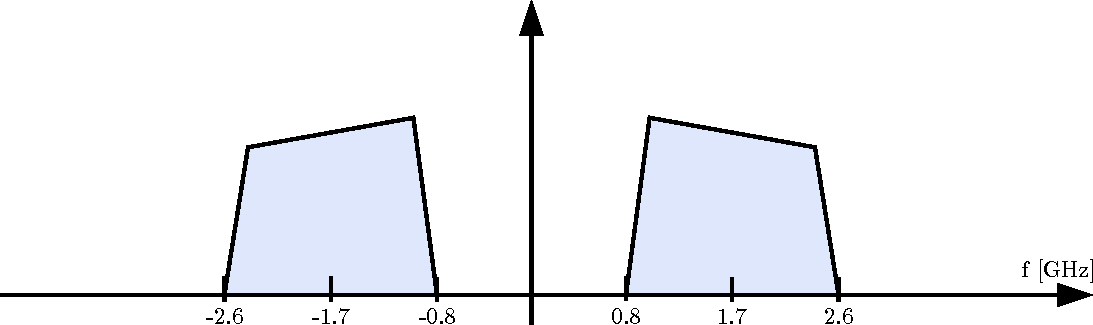
\includegraphics[width=0.8\textwidth]{figures/rx_0_freq_tx_if}
    \caption{\gls{TX} \gls{IF}}
    \label{fig:rx_0_frq_tx_if}
  \end{subfigure}
  \vspace{4ex} \\
  \begin{subfigure}{\textwidth}
    \centering
    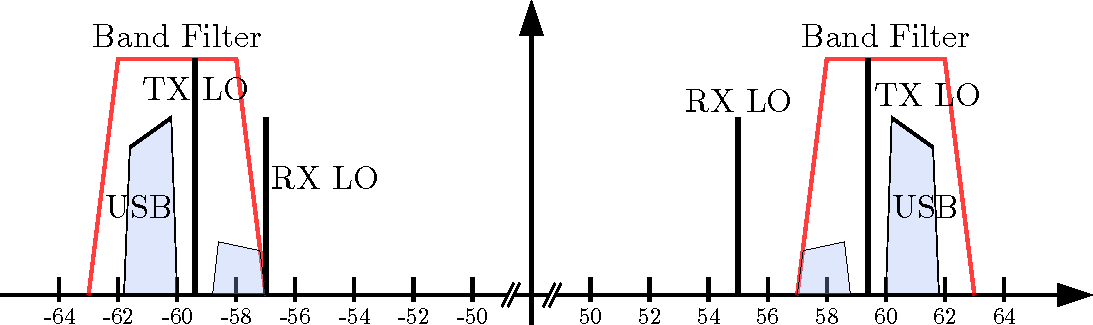
\includegraphics[width=0.8\textwidth]{figures/rx_0_freq_rf}
    \caption{\gls{RF}}
    \label{fig:rx_0_freq_rf}
  \end{subfigure}
  \vspace{4ex} \\
  \begin{subfigure}{\textwidth}
    \centering
    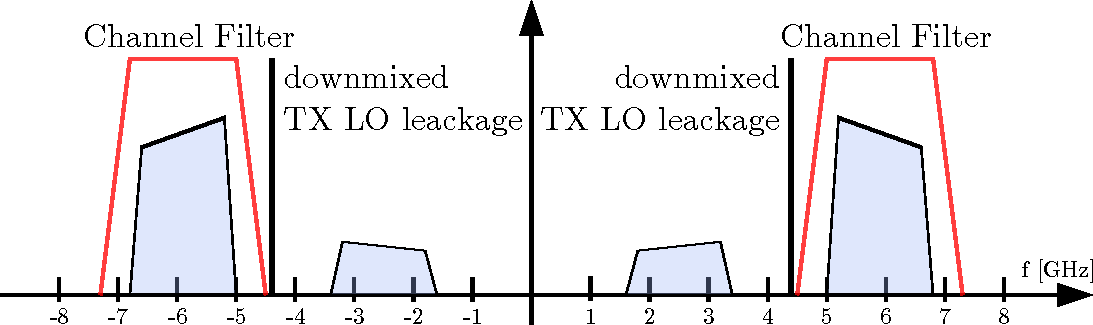
\includegraphics[width=0.8\textwidth]{figures/rx_0_freq_rx_if1}
    \caption{\gls{RX} high \gls{IF}}
    \label{fig:rx_0_freq_rx_if1}
  \end{subfigure}
  \vspace{4ex} \\
  \begin{subfigure}{\textwidth}
    \centering
    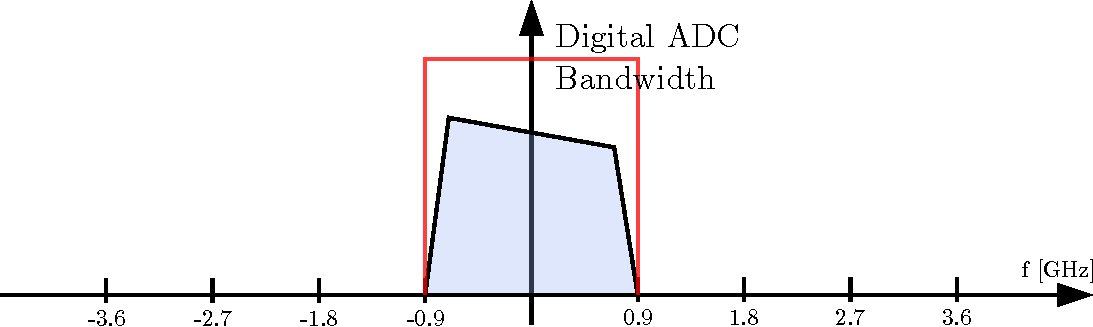
\includegraphics[width=0.8\textwidth]{figures/rx_0_freq_rx_if2}
    \caption{\gls{RX} low \gls{IF}}
    \label{fig:rx_0_freq_rx_if2}
  \end{subfigure}
  \caption{Quadrature Baseband Sampling Receiver in Frequency Domain}
  \label{fig:rx_0_freq}
\end{figure}

\subsection{Intermediate Frequency Sampling Receiver}
\label{sec:rx_1}
Next a different receiver architecture was considered which uses
$90^\circ$ couplers of image rejection as described in \secref{sec:rx_rf_1}
and than samples at an \gls{IF} aligned to the first Nyquist-zone as described
in \secref{sec:rx_adc_0}. \\

The block diagram is shown in \figref{fig:rx_1_bd}, the spectra in
\figref{fig:rx_1_freq} and the used frequencies in \tblref{tab:rx_1}. \\

The second \gls{IF} of $f_{\text{LO}_2} = 0.9$ was assigned such that
the 1.8 GHz wide signal fully falls into the first Nyquist-zone of
a single \gls{ADC} sampling at 3.6 GHz. Again a \gls{DC}-block
is used in front of the \gls{ADC}. Compared to the Quadrature Baseband
Sampling Receiver only half of the signal is lost this time since
the \gls{DC}-block now deletes the lowest frequency part of the signal
and not the central part symmetrically around zero. Also this error
can be completely avoided by using a symbol rate of slightly less
than 1.8 GHz. \\

The channel selection was than by a combination of two filter. First
a  high-pass filter (\figref{fig:rx_1_freq_rx_if1}) before
the second mixer removes signals between $f_{\text{RX LO}}$ and
$f_{\text{c}} - \frac{B}/{2}$ including the strong \gls{TX} \gls{LO}
leakage. The low-pass filter on the lower \gls{IF}
(\figref{fig:rx_1_freq_rx_if2}) is the second part of the channel
selection filter by preventing aliasing. \\

A drawback of this architecture is, that it requires a single \gls{ADC}
at the symbol speed $f_{s}$ instead of two \gls{ADC} channels at
$f_{s} / s$ used by the two other architectures. Such \gls{ADC} can,
as it was done in our setup, be build using a two channel \gls{ADC}
in interleaved mode. This may introduce many new errors as the not
perfect balancing of both channels and a high clock jitter frequency
component at $f_{s}$. \\

\begin{table}[h]
  \centering
  \begin{tabular}{|l|l|}
    \hline
    $f_{\text{TX IF}}$ & 1.7 GHz \\ \hline
    $f_{\text{TX LO}}$ & 58.2 GHz \\ \hline
    $f_{\text{RX LO}}$ & 57 GHz \\ \hline
    $f_{\text{RX IF}}$ & 2.9 GHz \\ \hline
    $f_{\text{LO}_2} $ & 2 GHz \\ \hline
    $f_c$           & 59.9 GHz \\ \hline
    Signal Bandwidth B & 1.8 GHz \\ \hline
    Number of \gls{ADC} channels & 1 \\ \hline
    Sample Rate $f_s$ & 3.6 GHz \\ \hline
  \end{tabular}
  \caption{Properties of Intermediate Frequency Sampling Receiver}
  \label{tab:rx_1}
\end{table}

\begin{figure}[h!]
  \centering
  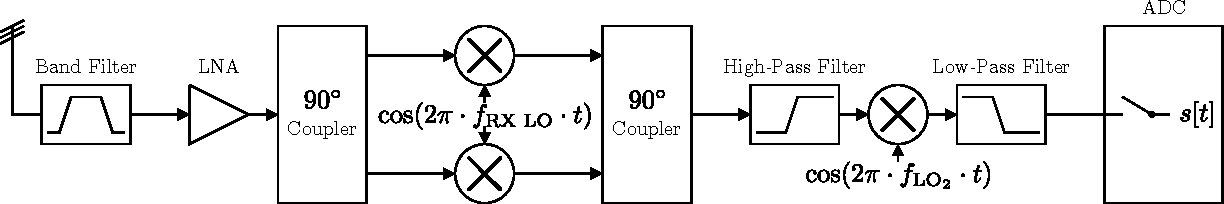
\includegraphics[width=\textwidth]{figures/rx_1_bd}
  \caption{Block Diagram of Intermediate Frequency Sampling Receiver}
  \label{fig:rx_1_bd}
\end{figure}

\begin{figure}[h!]
  \centering
  \begin{subfigure}{\textwidth}
    \centering
    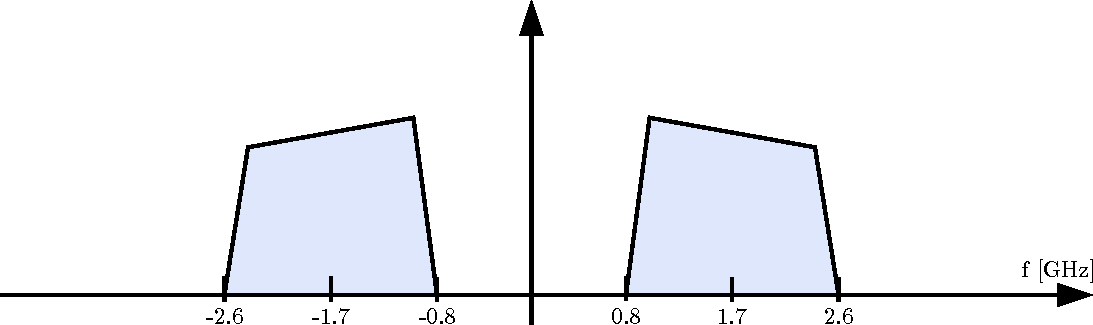
\includegraphics[width=0.8\textwidth]{figures/rx_1_freq_tx_if}
    \caption{\gls{TX} \gls{IF}}
    \label{fig:rx_1_frq_tx_if}
  \end{subfigure}
  \vspace{4ex} \\
  \begin{subfigure}{\textwidth}
    \centering
    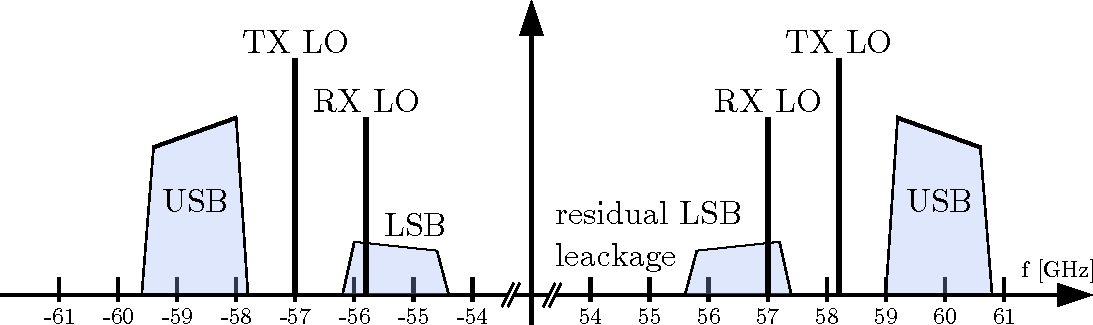
\includegraphics[width=0.8\textwidth]{figures/rx_1_freq_rf}
    \caption{\gls{RF}}
    \label{fig:rx_1_freq_rf}
  \end{subfigure}
  \vspace{4ex} \\
  \begin{subfigure}{\textwidth}
    \centering
    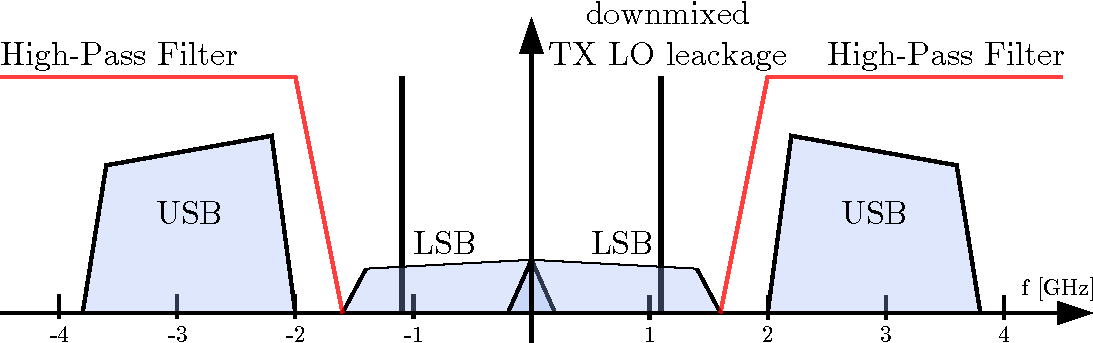
\includegraphics[width=0.8\textwidth]{figures/rx_1_freq_rx_if1}
    \caption{\gls{RX} high \gls{IF}}
    \label{fig:rx_1_freq_rx_if1}
  \end{subfigure}
  \vspace{4ex} \\
  \begin{subfigure}{\textwidth}
    \centering
    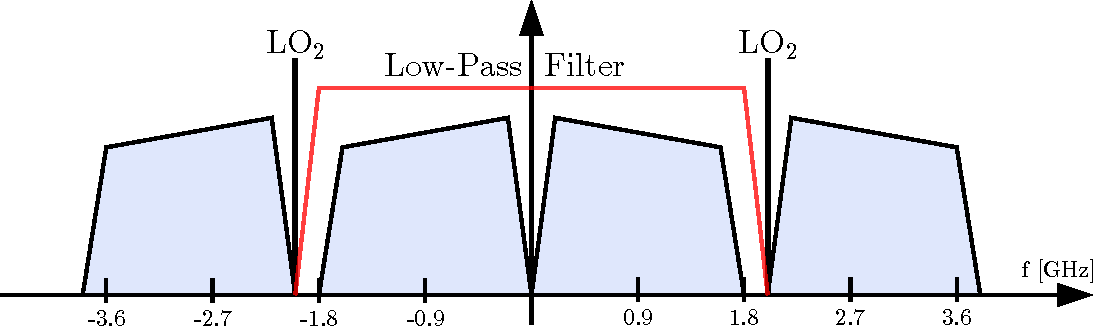
\includegraphics[width=0.8\textwidth]{figures/rx_1_freq_rx_if2}
    \caption{\gls{RX} low \gls{IF}}
    \label{fig:rx_1_freq_rx_if2}
  \end{subfigure}
  \caption{Intermediate Frequency Sampling Receive in Frequency Domain}
  \label{fig:rx_1_freq}
\end{figure}

\subsection{Quadrature Intermediate Frequency Sub-Nyquist Sampling Receiver}
\label{sec:rx_2}
The third receiver architecture, which was used for most measurements,
was motivated by having only very few components that can add noise
and errors due to non-linear terms. \\

It is, however, based on the assumption that no other channels of the
60 GHz spectrum are used except those, where we send residuals our self.
Therefor the very strong \gls{TX} \gls{LO} leakage and
the residual \gls{TX} \gls{LSBand} leakage are shown in all plots. \\

As shown in the block diagram in \figref{fig:rx_2_bd}, it only uses one
\gls{IF} where it performs Quadrature Sub-Nyquist Sampling as described
in \secref{sec:rx_adc_2}. \\

Since the to mixers of the 58-63 GHz converter work at much
higher frequencies than those used in the other architectures the
\gls{LO}-leakage and it's self-mixing is even more pronounced.
Because of that and probably also due to further component restrictions,
the converter is specified for an \gls{IF} of 1-5 GHz as noted in
\secref{sec:comp_sivers}.
Since the desired signal with has a full bandwidth of 1.8 GHz results
in an \gls{RX} \gls{IF} between 1.0 and 2.8 GHz, this just meets
this specifications. \\

The \gls{ADC} 12d1800 has an analog bandwidth of typically 2.8 GHz
as described in \secref{sec:comp_adc}.
Therefor the upper limit of the 2.8 GHz of \gls{RX} \gls{IF} meets this
requirement as well. \\

After the $f_{\text{RX IF}}$ is fully defined by this constraints, the
$f_{\text{TX LO}}$ and $f_{\text{RX LO}}$ have to be looked at.
As we can see in \figref{fig:rx_2_freq_a_0} the \gls{TX} \gls{LO}
leakage will be at $q = f_{\text{RX LO}} - f_{\text{TX LO}}$. Te be optimally
suppressed by the channel filter, this difference should be as small
as possible. On the other hand, the residual \gls{TX} \gls{LSBand} signal
we be separated from the desired \gls{TX} \gls{USBand} signal by $2 \cdot q$
which demands for $q \geq \frac{f_s}{2}$. \\
Unfortunately only one of this constraints can be meet. Since the \gls{TX}
\gls{LO} leakage is much stronger then the residual \gls{TX} \gls{LSBand}
leackage, the difference was chosen to be $q = 0.7 GHz$ resulting in the
\gls{TX} \gls{LO} leackage to be well suppressed by the channel filter while
the residual \gls{TX} \gls{LSBand} signal overlaps only 0.6 GHz. \\

The absolute value of $f_{\text{RX LO}}$ was then chosen such that the
carrier frequency $f_c = 60.1 \text{GHz}$ is in the middle of the
converter's \gls{RF} specification and the residual \gls{TX} \gls{LSBand}
54.9 GHZ well outside. \\

Consequently $f_{\text{TX IF}} = f_c - f_{\text{TX LO}} = 2.6 \text GHz$ which
meets the \gls{IF} specification of the converter as well. \\

The receiver first mixes \gls{RF} signal $r(t)$ with a the local oscillator
at $f_{\text{RX LO}}$ and a $90^\circ$ shifted version of this oscillator
as shown in \figref{fig:rx_adc_1_freq_cos} and \figref{fig:rx_adc_1_freq_sin}.
Again the frequency components at $\pm (f_c + f_{\text{RX LO}})$ are
automatically filtered and noted as a low-pass filter LP.
See: \eqref{eq:rx_2_a_0}, \eqref{eq:rx_2_a_1},
\figref{fig:rx_2_freq_a_0} and \figref{fig:rx_2_freq_a_1} \\

\begin{subequations}
  \begin{alignat}{2}
    a_0(t) &= \text{LP}\{r(t) \cdot \cos(2\pi \cdot f_{\text{RX LO}} \cdot t)\}
    \label{eq:rx_2_a_0} \\
    a_1(t) &= \text{LP}\{r(t) \cdot \sin(2\pi \cdot f_{\text{RX LO}} \cdot t)\}
    \label{eq:rx_2_a_1}
  \end{alignat}
\end{subequations}

Next the channel filter implemented as a band pass filter is applied.
The resulting signals $b_0(t) = \text{BP}\{a_0(t)\}$ and
$b_1(t) = \text{BP}\{a_1(t)\}$ are shown in \figref{fig:rx_2_freq_b_0}
and \figref{fig:rx_2_freq_b_1}. \\

Then the two analog signals $b_0(t)$ and $b_1(t)$ are sampled by two
separate \gls{ADC} channels as noted in \eqref{eq:rx_2_c_0} and
\eqref{eq:rx_2_c_1} and drawn in \figref{fig:rx_2_freq_c_0}
and \figref{fig:rx_2_freq_c_1}. \\

\begin{subequations}
  \begin{alignat}{2}
    c_0[k] &= \int_{-\infty}^{\infty}
    b_0(t) \cdot \delta\left(t - \frac{k}{f_s}\right) \; \text{d}t
    \;\; \forall k \in \mathbb{Z}
    \label{eq:rx_2_c_0} \\
    c_1[k] &= \int_{-\infty}^{\infty}
    b_1(t) \cdot \delta\left(t - \frac{k}{f_s}\right) \; \text{d}t
    \;\; \forall k \in \mathbb{Z}
    \label{eq:rx_2_c_1}
  \end{alignat}
\end{subequations}

Next the two digital signals $c_0[k]$ and $c_1[k]$ are interpreted as one
complex discrete signal $d[k] = c_1[k] + j \cdot c_0[k]$ as shown in
\figref{fig:rx_2_freq_d}. \\

To get a better picture of how the resulting signal looks like,
\figref{fig:rx_2_freq_e} shows $e[k] = -j \cdot d[k]$. Also the signal
originating from the \gls{TX} \gls{LSBand} residual is colored yellow
while to desired signal stays blue.
As noticed before, this architecture does not fully suppress neighbouring
channels. \\

The get the correct baseband signal $f[k]$, $e[k]$ has to be shifted by
$f_{\text{RX IF}} - f_s = 100 \; \text{MHz}$:

\begin{align}
  f[k] = e[k] \cdot \exp\left(-2\pi \cdot j \cdot
  \frac{f_{\text{RX IF}} - f_s}{f_s} \cdot k \right)
  \;\; \forall k \in \mathbb{Z}
\end{align}

\begin{table}[h]
  \centering
  \begin{tabular}{|l|l|}
    \hline
    $f_{\text{TX IF}}$ & 2.6 GHz \\ \hline
    $f_{\text{TX LO}}$ & 57.5 GHz \\ \hline
    $f_{\text{RX LO}}$ & 58.2 GHz \\ \hline
    $f_{\text{RX IF}}$ & 1.9 GHz \\ \hline
    $f_c$            & 60.1 GHz \\ \hline
    Signal Bandwidth B & 1.8 GHz \\ \hline
    Number of \gls{ADC} channels & 2 \\ \hline
    Sample Rate $f_s$ & 1.8 GHz \\ \hline
  \end{tabular}
  \caption{Properties of Quadrature Intermediate Frequency
    Sub-Nyquist Sampling Receiver}
  \label{tab:rx_2}
\end{table}

\begin{figure}[h!]
  \centering
  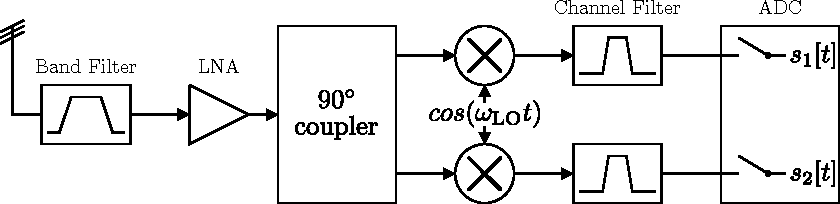
\includegraphics[width=\textwidth]{figures/quad_if_rx_block_diagram}
  \caption{Block Diagram of Quadrature Intermediate Frequency Sub-Nyquist Sampling Receiver}
  \label{fig:rx_2_bd}
\end{figure}

\begin{figure}[h!]
  \centering
  \begin{subfigure}{0.45\textwidth}
    \centering
    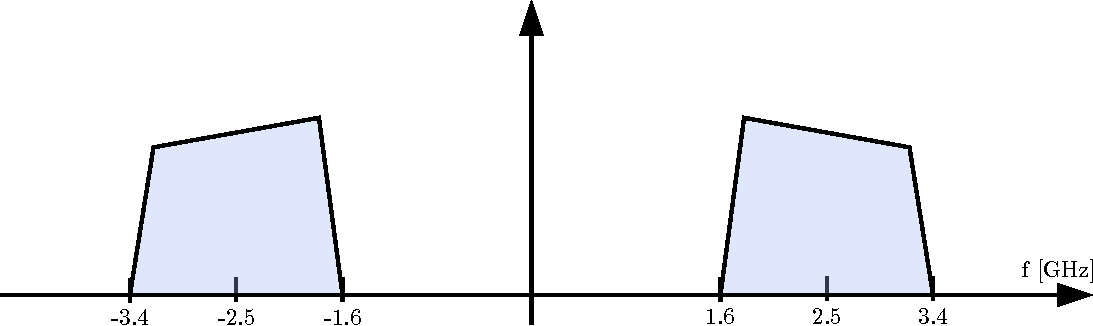
\includegraphics[width=\textwidth]{figures/rx_2_freq_tx_if}
    \caption{\gls{TX} \gls{IF}}
    \label{fig:rx_2_freq_tx_if}
  \end{subfigure}
  ~
  \begin{subfigure}{0.45\textwidth}
    \centering
    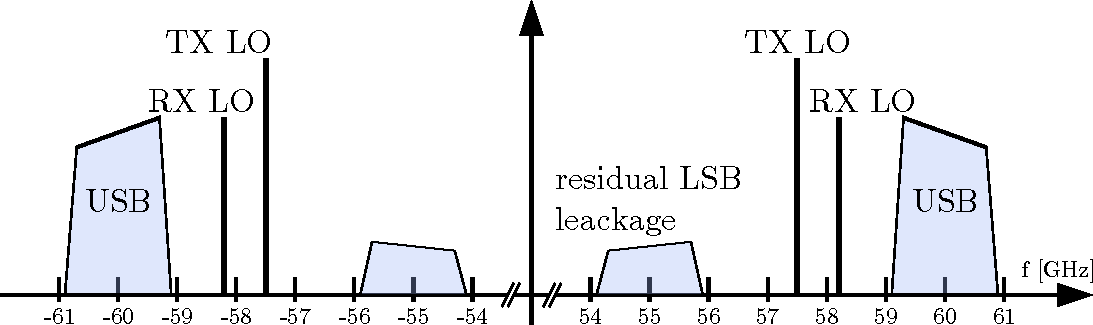
\includegraphics[width=\textwidth]{figures/rx_2_freq_rf}
    \caption{$r(t)$ : \gls{RF}}
    \label{fig:rx_2_freq_rf}
  \end{subfigure}
  \vspace{4ex} \\
  \begin{subfigure}{0.45\textwidth}
    \centering
    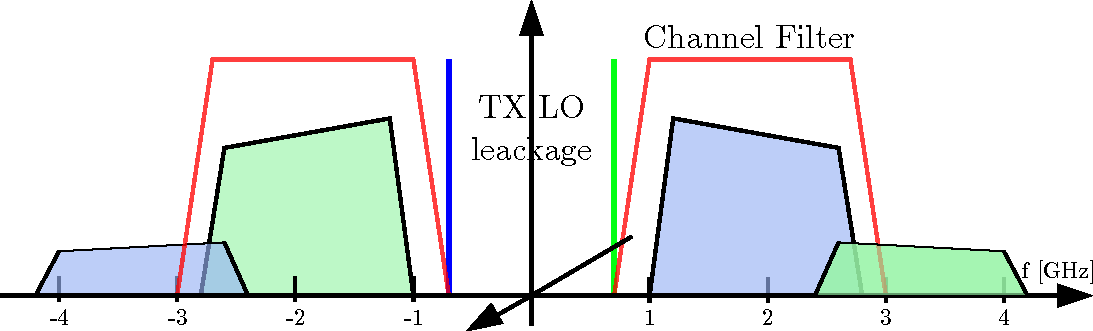
\includegraphics[width=\textwidth]{figures/rx_2_freq_a_0}
    \caption{$a_0(t) = \text{LP}\{r(t) \cdot \cos(2\pi \cdot f_{\text{RX LO}} \cdot t)\}$}
    \label{fig:rx_2_freq_a_0}
  \end{subfigure}
  ~
  \begin{subfigure}{0.45\textwidth}
    \centering
    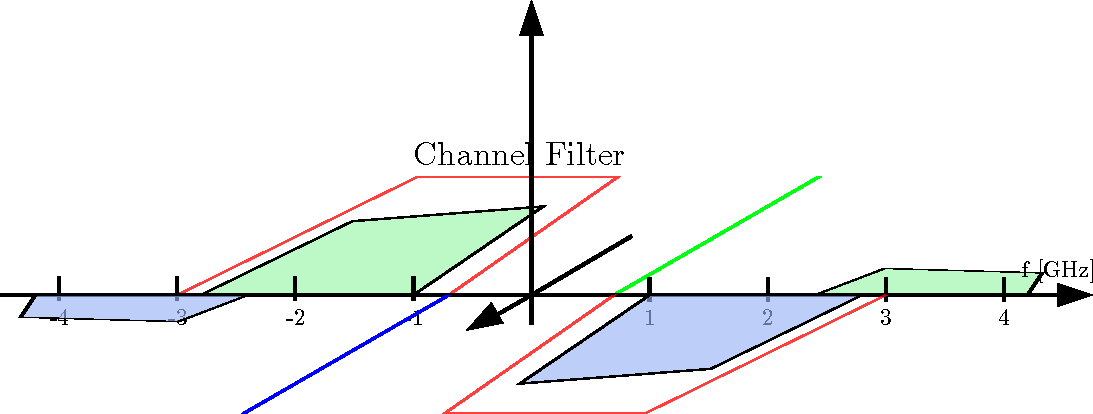
\includegraphics[width=\textwidth]{figures/rx_2_freq_a_1}
    \caption{$a_1(t) = \text{LP}\{r(t) \cdot \sin(2\pi \cdot f_{\text{RX LO}} \cdot t)\}$}
    \label{fig:rx_2_freq_a_1}
  \end{subfigure}
  \vspace{4ex} \\
  \begin{subfigure}{0.45\textwidth}
    \centering
    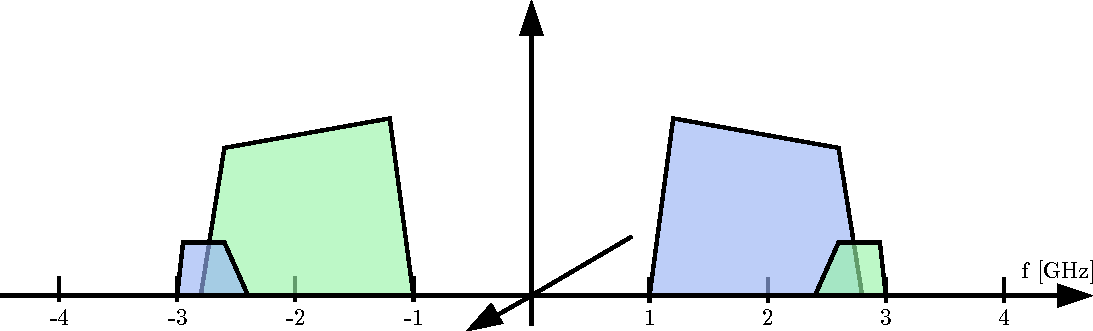
\includegraphics[width=\textwidth]{figures/rx_2_freq_b_0}
    \caption{$b_0(t) = \text{BP}\{a_0(t)\}$}
    \label{fig:rx_2_freq_b_0}
  \end{subfigure}
  ~
  \begin{subfigure}{0.45\textwidth}
    \centering
    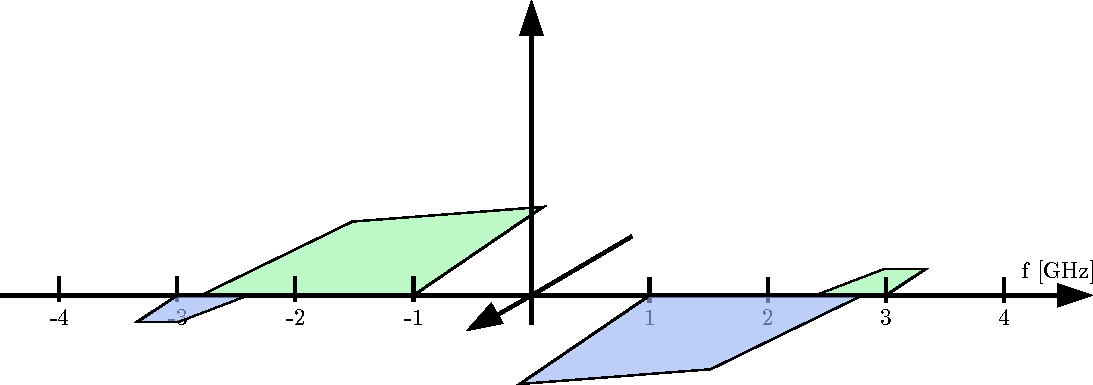
\includegraphics[width=\textwidth]{figures/rx_2_freq_b_1}
    \caption{$b_1(t) = \text{BP}\{a_1(t)\}$}
    \label{fig:rx_2_freq_b_1}
  \end{subfigure}
  \vspace{4ex} \\
  \begin{subfigure}{0.45\textwidth}
    \centering
    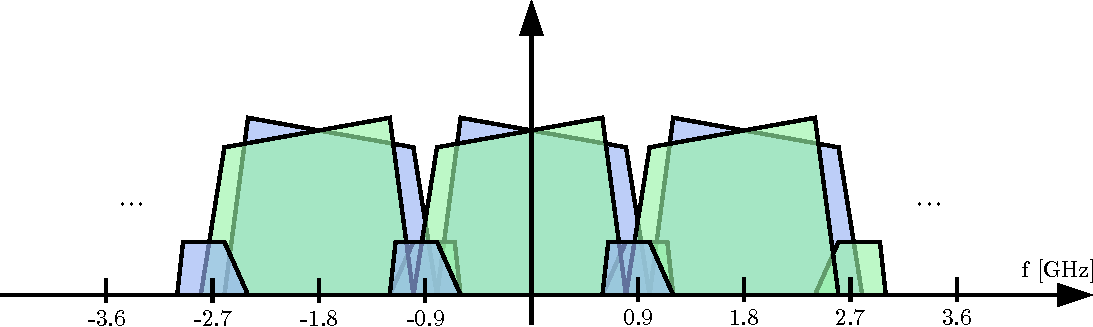
\includegraphics[width=\textwidth]{figures/rx_2_freq_c_0}
    \caption{$c_0[k] = b_0(k/f_x)$}
    \label{fig:rx_2_freq_c_0}
  \end{subfigure}
  ~
  \begin{subfigure}{0.45\textwidth}
    \centering
    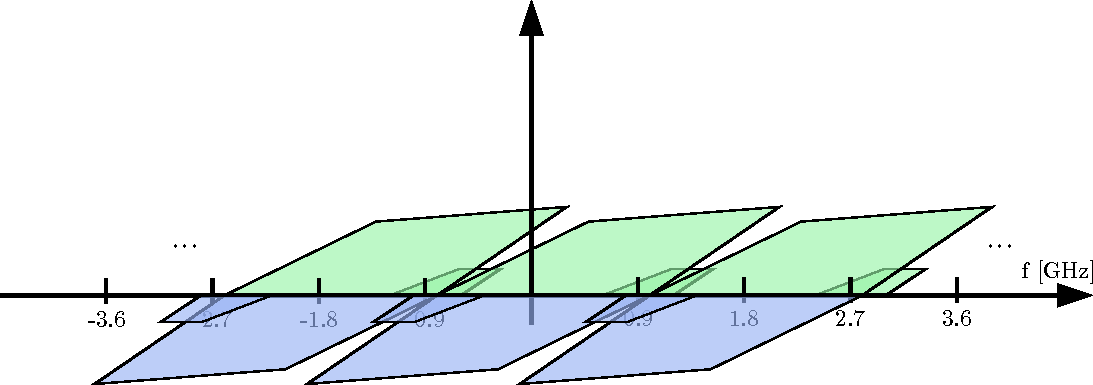
\includegraphics[width=\textwidth]{figures/rx_2_freq_c_1}
    \caption{$c_1[k] = b_1(k / f_x)$}
    \label{fig:rx_2_freq_c_1}
  \end{subfigure}
  \vspace{4ex} \\
  \begin{subfigure}{0.45\textwidth}
    \centering
    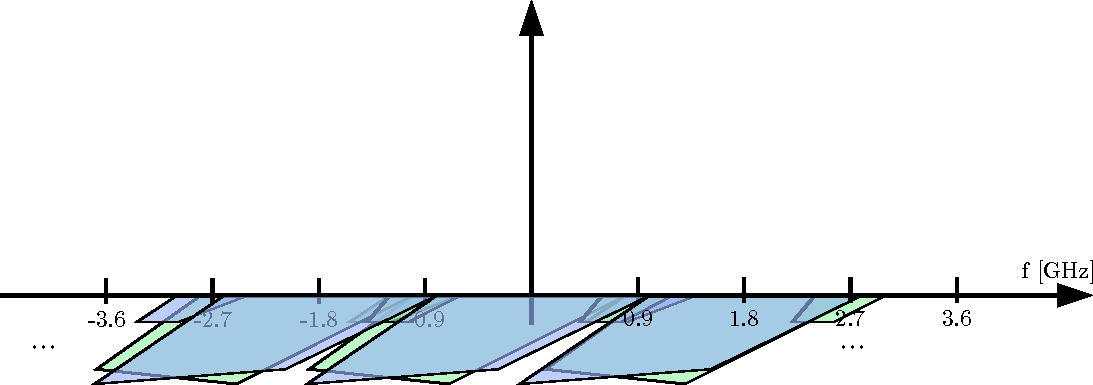
\includegraphics[width=\textwidth]{figures/rx_2_freq_jc0}
    \caption{$j \cdot c_0[k]$}
    \label{fig:rx_2_freq_jc0}
  \end{subfigure}
  ~
  \begin{subfigure}{0.45\textwidth}
    \centering
    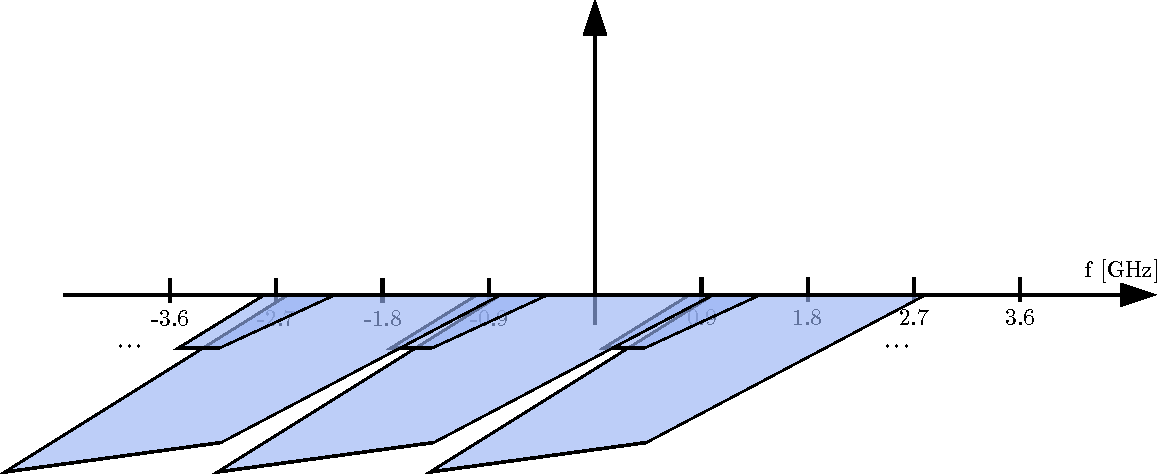
\includegraphics[width=\textwidth]{figures/rx_2_freq_d}
    \caption{$d[k] = c_1[k] + j \cdot c_0[k]$}
    \label{fig:rx_2_freq_d}
  \end{subfigure}
  \vspace{4ex} \\
  \begin{subfigure}{0.45\textwidth}
    \centering
    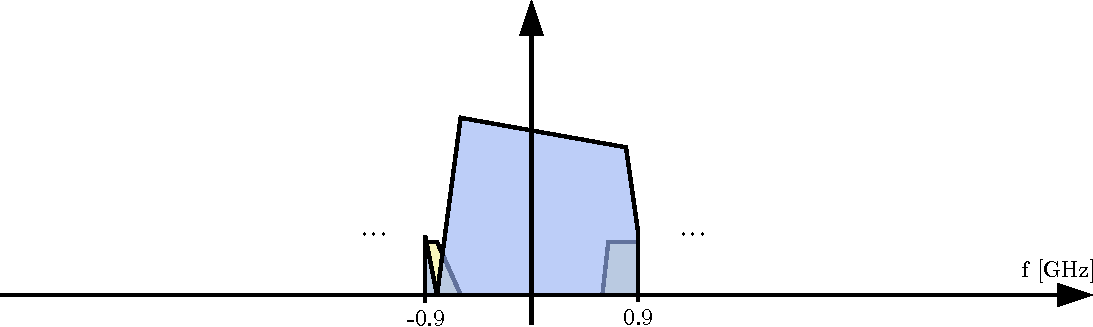
\includegraphics[width=\textwidth]{figures/rx_2_freq_e}
    \caption{$e[k] = -j \cdot d[k]$}
    \label{fig:rx_2_freq_e}
  \end{subfigure}
  \caption{Quadrature Intermediate Frequency Sub-Nyquist Sampling Receiver
    in Frequency Domain}
  \label{fig:rx_2_freq}
\end{figure}

%%  LocalWords:  Sivers IMA sivers USBand LSBand DAC coupler rx rf bd
%%  LocalWords:  interferer SNR LNA convolve Couplers couplers Hs Hb
%%  LocalWords:  hilbert Baseband baseband adc eq ja Nyquist Meca ISI
%%  LocalWords:  jitter

\chapter{Communication System and its simulation}


\begin{itemize}
\item 802.11ad oriented receiver
\item but non standard supplient
\item aim: show that big datarates are possible
\item aim: use to investigate phase noise behaviour and find other non ideal effects
\item perfomance limiting impairments
\end{itemize}

\section{Modulation and Pulse Shaping Scheme}
\begin{itemize}
\item bpsk / QAM
\item root raised cosine filter for pulse shaping
\end{itemize}


\section{Frame strucutre}
\begin{itemize}
\item 802.11ad oriented
\item ZEROS FES CES FIRST\_PES DATA PES DATA PES ... ZEROS
\item Explain reason of all fields
\item Explain cyclic properties
\end{itemize}

\section{Frequency offset estimation and correction}

\section{Phase noise estimation and correction}
\begin{itemize}
\item Cite phase noise measurements of Radoslav
\item Explain how to estimate and correct it
\item reference to own results in later chapter
\end{itemize}

\section{Simulation}
\begin{itemize}
\item General simulation flow using Matlab
\item Simulated scenarios:
  \begin{itemize}
  \item Baseband receiver
  \item Simulated 90 deg coupler using hilbert transform
  \item hardware baseband QI receiver
  \item hardware intermediate frequency QI receiver
  \end{itemize}
\item Interface to AWG
\item Interface to Oscilloscope
\item Interface to FPGA
\item Replace more and more by hardware
\end{itemize}


\chapter{FPGA}
\label{chap:fpga}
A powerful Virtex-7 \gls{FPGA} Evaluation board VC707
was used to for the real time signal processing.
For the experiments performed in this thesis
the data from the \gls{ADC} is acquired, stored in real time
and than passed to Matlab running on a personal computer.
This allowed to both test the analog part of the system
while keeping the fast implementation speed and flexibility of Matlab
to test the rest of the digital signal processing steps of the receiver.
Nevertheless the architecture was chosen such that it is now easy
to step by step move parts of the signal processing from Matlab to the
\gls{FPGA}. \\

\section{Architecture Overview}
The three main tasks of the digital design are first do interface
the \gls{ADC} and acquire its data, then to store them on a
\gls{DDR} \gls{RAM} and finally to allow a computer to
slowly download it. \\

As shown in \figref{fig:fpga_architecture_overview} the most important
modules of the design are the Adc12d1800 which interfaces the
\gls{ADC}, Ram which uses a \gls{DDR}3-\gls{RAM} to store the data
and Microblaze, a soft-core processor, which controls the
\gls{USB} 2 data download. Data2Ram is the interface logic used
to connect the \gls{ADC} directly to the \gls{RAM}. Later the receiver logic,
starting with frame synchronization could be implemented
at this place. AxiSlave implements an interface between the
\gls{AXI}-Bus used by the Microblaze processor and the custom
Ram module. \\

In the following sections each of this modules is shortly described followed
by some insights how clocking and reset is implemented. \\

\begin{figure}[ht]
  \centering
  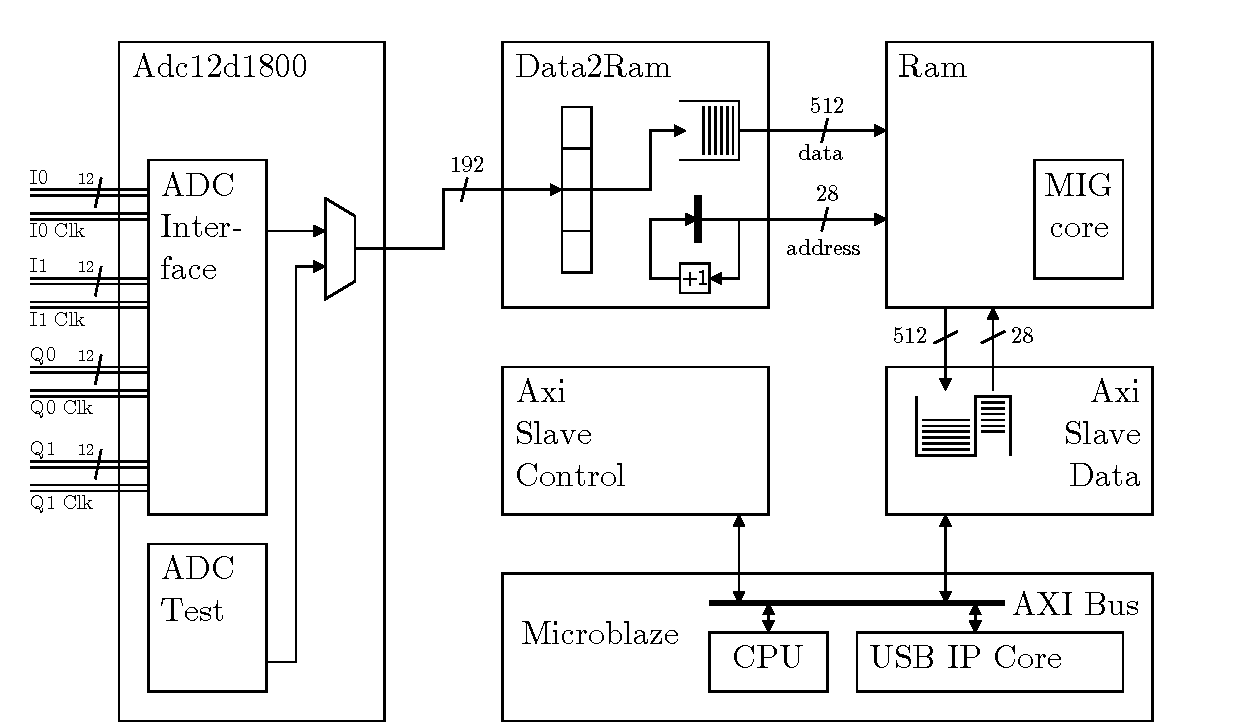
\includegraphics[width=\textwidth]{figures/fpga_architecture_overview}
  \caption{Overview of the architecture}
  \label{fig:fpga_architecture_overview}
\end{figure}

\section{Req/Ack Protocol}
\label{sec:fpga_reqack}
Between most modules a simple communication protocol is used that allows
one way communication whenever the sender and the receiver are both
ready. As a consequence all modules have to be stallable. By only using
one such protocol arbitrary modules can often be connected
without any additional glue logic. \\

The protocol requires the sender to provide a \acrfull{req} output which
is asserted if it has data to send. The receiver provides a \acrfull{ack}
output to confirm that it is ready to receive the data.
Acknowledge can only be applied when \gls{req} is asserted.
Data is transferred whenever there is a positive clock edge and
\gls{req} and \gls{ack} are both asserted (high). \\

Because the acknowledge output of a receiver by definition always depends on the
\gls{req} input of a receiver, this can result in long chains of routing and
\gls{LUT} resources when connecting multiple such modules.
Therefor a simple so called \gls{req}/\gls{ack}-breaker is used which adds one
register into the data path. This results in one cycle delay but makes the
\gls{ack} signal depending on a local register only and not on the
\gls{req} signal. \\

This has also the advantage that long routing distances can be separated by
inserting registers into the data and control path. \\

\section{Data Acquisition}
\label{sec:fpga_adc}

The \gls{ADC} Reference Board (see \secref{sec:comp_adc}) is connected
to the Virtex-7 evaluation board (see \secref{sec:comp_virtex7})
using one of the two \gls{FMC} plugs.
A listing of all connections can be found in \secref{sec:app_adc_fpga_con}. \\

Data acquisition is done by the module Adc12d1800. In our case the ADC is
configured to sample two channels, an in-phase and a quadrature phase channel,
at up to 1.8 GHz or to sample one channel at 3.6 GHz.
The nominal resolution is 12 bits. This results in a total bandwidth of
$5.4 \text{GB}/\text{s}$. \\
Since 1.8 GHz and especially 3.6 GHz is far beyond what the IO-Pads of all
\glspl{FPGA} \todo{reference needed} and most \glspl{ASIC} can handle,
the ADC can output on 4 parallel streams of 12 bits each. \\

Since this 4 streams might be routed with different wire lengths on a \gls{PCB}
each stream has it's own clock which is aligned to the data.
In order to half the maximum frequency of the clock line,
the data change on positive and negative clock edges (\gls{DDR}). \\

At full speed, this results in a switching frequency of 450 MHz for all data
and clock lines. To support this high speed while reducing power consumption,
and the influence of noise compared to classical \gls{CMOS} signaling,
\gls{LVDS} is used. \\

Since the maximum clock frequencies of the Virtex \glspl{FPGA} for logic
including \gls{LUT} slices and medium to high fan-outs
are limited to around 200 to 300 MHz, the input stream needs to be further
parallelised. This design uses a frequency of 250 MHz to output
the data of the \gls{ADC} for further processing. At this frequency
the only $4\;\text{ns}$ are available between clock edges which is exceeded
easily as soon as a signal is routed far across the \gls{FPGA} die,
has a fan-out of more than about 4, when crossing clock domains which leads
to clock skew or by more than about 3 logic slices between registers.
This makes the \gls{FPGA} design challenging since often multiple
complete synthesis, map, place \& route and timing analysis runs are
needed to find a design that meets timing. \\

As shown in \figref{fig:fpga_adc} the implemented design uses
a total of 4 stages to parallelise and centralize the data to
one single data stream. \\

\begin{figure}[ht]
  \centering
  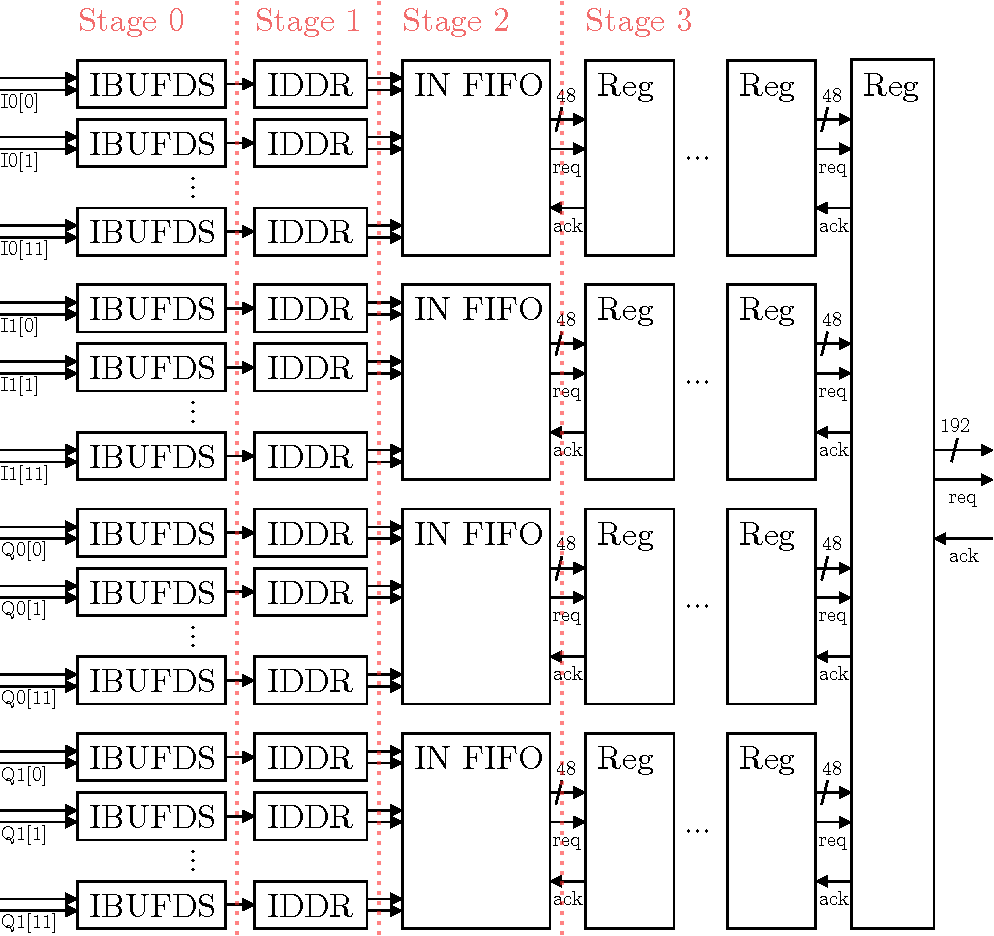
\includegraphics[width=\textwidth]{figures/fpga_adc}
  \caption{Data path of the \gls{ADC} module}
  \label{fig:fpga_adc}
\end{figure}

\subsection{Stage 0: Differential to Single-ended Conversion}
Each of the 12 bits and the clock of the 4 streams arrive at at the input bank
of the \gls{FPGA} at two neighbouring pads forming a \gls{LVDS} pair.
First this differential signal is converted to a single ended signal using
\gls{IBUFDS} primitives located next
to the pads. \\

This results in $4 \times 12$ bits of single ended double data rate
signals plus 4 single ended clocks at up to 450 MHz. \\

\subsection{Stage 1: Double Data Rate to Single Data Rate Conversion}
\label{sec:fpga_adc_s1}
Next the first parallelisation step is performed by outputting two new
bits on every positive clock edge instead of one on positive and one on negative
clock edges. The Virtex-7 \gls{FPGA} have a dedicated hardware primitive
called \gls{IDDR} for this.
This primitives are placed next to the differential input buffers
and are automatically mapped correctly by the Xilinx tools. \\

This results in $4 \times 24$ bits of single ended single data rate
signals plus 4 single ended clocks at up to 450 MHz. \\

\subsection{Stage 2: Input FIFO}
Since 450 MHz is still beyond what can be routed through the general
routing resources and captured by registers, Xilinx added a special
\gls{INFIFO} primitive directly into the IO-bank which can parallelise the data
by a factor of two.
This primitive has a total of ten 4 bit wide input buses.
The primitive can be configured to concatenate two consecutive input words
to one 8 bit wide output word and therefore provides a total of
ten 8 bit wide output words. \\

Four such \gls{INFIFO} are available for each
input/output bank consisting of a total of 50 pads aligned in a single row.
In our design each of the four 24-bit input streams is located at a separate
input/output bank and is routed to the inputs of one \gls{INFIFO} primitive.
Since the timing only holds if the \gls{INFIFO} instance in the middle of the bank
is used. Because mapping tools prefer other locations depending on the
routing of the outputs, all those \gls{INFIFO} primitives where manually constrained
to the correct location. \\

These \gls{INFIFO} also support an independent input and output clock.
As input clock the clock signals provided by the \gls{ADC} are each fed
into a so called \gls{MMCME2ADV}.
This allows to arbitrarily shift the phases of the clocks to ensure
correct data capturing. The same clock was also used for the
\gls{IDDR}-registers described in \secref{sec:fpga_adc_s1}. \\

For each input bank one such clock manager exists. To ensure that
always the one next to the input clock pads and the \gls{INFIFO} is
used, the four MMCME2\_ADV instances are also manually constrained to
one specific location. \\

This results in $4 \times 48$ bits of single ended single data rate signals. \\

\begin{figure}
  \centering
  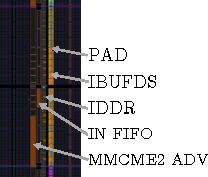
\includegraphics{figures/adc_input_bank}
  \caption{View of the physical location of the primitives forming the
    \gls{ADC} interface on the \gls{FPGA}}
  \label{fig:adc_input_bank}
\end{figure}

\subsection{Stage 3: Centralization and Reordering}
\label{sec:fpga_adc_s3}
All previous stages kept the four input streams separated
and were placed close to four input bank spread across the whole die.
Hence the data has to be routed to one place first.
This is done by allocating three req/ack breakers in series for each of the
four channels.
This induces a high flexibility to the tools in allocating routing
resources and putting registers in between. \\

The four last \gls{req}/\gls{ack} breakers of the four channels are then connected
to one single \gls{req}/\gls{ack} breaker which forms the final output of the
\gls{ADC} module. The data is ordered in such a way, that the final 192 bit
wide output vector is formatted as follows:
\[Q_7\;I_7\;Q_6\;I_6\;Q_5\;I_5\;Q_4\;I_4\;Q_3\;I_3\;Q_2\;I_2\;Q_1\;I_1\;Q_0\;I_0\]
Where $Q_t$ and $I_t$ are the quadrature channel respectively in-phase channel
12 bit words at time $t$.
The index $t$ is the time step. A higher number means later in time.
All the words are formatted with \gls{MSB} first. \\

This results in $1 \times 192$ bits of single ended single data rate signals. \\

\subsection{Test pattern generator}
For debugging purposes the \gls{ADC} interface has a built in test pattern
generator which outputs 16 words of 12 bit numbers in parallel such that
when lining them up to 192 bit vectors this results in a continuous count.

\section{Storage}
\label{sec:fpga_storage}
Whenever a positive edge is detected on the trigger input or the trigger
button is pressed, the \gls{RAM} is completely overwritten with a new run of
\gls{ADC} samples. \\

The arm signal (see \figref{fig:fpga_architecture_overview}) is deasserted
by the \gls{MB} processor while a download option is in process
(see \secref{sec:fpga_download}) to avoid mixing up multiple runs. \\

The used \gls{RAM} module MT8JTF1286Hz is a standard \acrshort{DDR}3 \gls{RAM}
and offers a total of 1 GiB of space spread across 8 banks of 128 MiB each.
This allows for parallel data transfers of 64 bits at speed of up to 800 MHz
resulting in a maximal bandwidth of $12.8 \text{GB}/\text{s}$. \\

Very similar to the \gls{ADC} data acquisition module (\secref{sec:fpga_adc})
this high clock rates can only be used very close to the input/output banks
and not for further routing and processing in the \gls{FPGA}.
For that purpose Xilinx provides a \gls{IP} core that on one end is connected
to the pads of the \gls{RAM} module and on the other side offers a user
friendly \gls{UI} on in slower clock frequency.
It does so by taking care of address generation, refreshing the volatile
memory and scheduling read and write options. \\

Because place \& route turned out to be difficult at the maximal speed
of 800 MHz I used only 500 MHz as \gls{RAM} clock rate.
When configuring the core to use a 1:4 multiplexing, the \gls{UI} runs
at 125 MHz, has a $4 \cdot 2 \cdot 64 = 512$ bits wide data bus
and a maximal bandwidth of $8 \text{GB}/\text{s}$. This is still slightly
higher than bandwidth of the \gls{ADC} and therefore allows real-time
storage of all data. Since there is 1 GiB \gls{RAM}
a total of $\approx 3.6 \cdot 10^8$ complex samples can be saved. This
takes $\approx 190 \text{ms}$ at full \gls{ADC} speed. \\

Experiments showed that it is possible to consecutively writing to all
addresses without the \gls{MIG} core stalling for refresh options.
Whenever, during the write requests, one sole read request
is performed, the \gls{UI} of the \gls{MIG} core stalls for about 11
cycles. This is not an issue as in our case we first write
to all addresses, then stop writing and read out a part of the memory
at much lower speeds (see \secref{sec:fpga_download}). \\

Since the \gls{ADC} module outputs the data at 250 MHz in a 192 bit
wide vector and the \gls{RAM} module can write 512 bit wide vectors
at only 125 MHz a bus converter is used which concatenates 192 bits
words until at least 512 bits are available. Behind this converter
a \gls{FIFO} memory is added to cross the clock boundary and to be able
to hold some samples when the \gls{MIG} user interface stalls. \\

During implementation care has to be exercised to the mask bits,
which are designed to prevent parts of the 64 bit written in parallel to be
overwritten and therefor allow for partial writes without first performing
a read operation. Accidentally having these pins stuck at 1 due to
not connecting them prevents initialization and further reads from
working. \\

\section{Download}
\label{sec:fpga_download}
For further analysis and processing of the data captured by the \gls{ADC}
it is sent to a personal computer.
Different options for downloading the 1 GiB of data from the \gls{FPGA}
to a computer were considered: \\

The simplest implementation would be to use the CP2103GM
\acrshort{USB}-to-\acrshort{UART} bridge \gls{IC} soldered on the VC707.
Since it's maximal baud rate is limited to $1 \text{Mbit}/\text{s}$
a complete download of 1 GiB would take about 18 minutes which was
considered to be too slow. \\

Next the Tri-Speed Ethernet \gls{PHY} device was considered.
The high data rates of up to $1 \text{Gbit}/\text{s}$ and the versatility
of being able to connect it to existing network infrastructure made
it look perfect for the job. The lack of a good reference design and
availability of open cores to connected to the \gls{PHY} via
\gls{SGMII} as well as the effort needed to implement
the network and transport (\gls{INetP}/\gls{UDP}) layer
led to the third solution. \\

The VC707 also includes a USB3320 USB 2.0 ULPI device and Xilinx provides
a out of the box \gls{IP} core to connect to it. The theoretical maximal
raw bandwidth of $60 \text{MB}/\text{s}$ would allow for a relatively fast
download. Also \gls{USB} is very common way to connect to modern laboratory
equipment.

\subsection{Microblaze Soft-core processor}
Since the initialization, control logic and packet formatting
used to implement the \gls{USB} slave device can much easier be implemented
in software than using look-up tables and \glspl{FSM} a
\gls{MB} soft-core processor was configured into the \gls{FPGA}. \\

As primary system bus to connect the processor to the following peripherals
a \gls{AXI} bus is used:
\begin{itemize}
\item RS232 \gls{UART} for status and debug outputs
\item 4 Bit output to control debug \glspl{LED}
\item USB 2 controller
\item An interrupt controller
\item The custom 60 GHz receiver peripheral
\end{itemize}

Since the \gls{RAM} module had to be optimized for best write performance
as described in \secref{sec:fpga_storage} not the standard Xilinx \gls{IP}
core to interface the \gls{MIG} core to the \gls{AXI} bus was used.
Instead a custom \gls{AXI} peripheral was implemented which allows to
control and monitor the data acquisition and a second peripheral allows
for memory mapped read access of the \gls{RAM} by the \gls{MB}. \\

For simplicity the \gls{DMA} unit of the \gls{USB} peripheral was not used.
Instead the data was first read from the custom 60 GHz peripheral
by the \gls{MB} processor and then written to \gls{USB} peripheral.
This allows for data transfer rates of about $16 \text{MB} / \text{s}$
which is already fast enough. \\

\subsection{Protocol}
To manage the communication between the host computer and the \gls{USB} device
implemented by the \gls{MB} a simple protocol was defined.
It involves 5 endpoints as they are defined by the \gls{USB}2 standard.
Only the Hi-Speed mode of \gls{USB}2 is supported. The slower Full Speed mode
is not supported. \\

Endpoint 0 is a standardized control endpoint. It's purpose is to
enumerate the bus\footnote{give the slave a unique address} and to provide the
host computer with information about basic parameters and the other endpoints
implemented by the slave. It's exact behaviour is defined by the
``Chapter 9 USB Device Framework'' of the \gls{USB}2 standard \todo{add reference}. \\

Endpoint 1 is used to transfer binary raw data from the computer to the \gls{FPGA}
while endpoint does the same into the other direction. They both use the maximal
possible packet size of 512 byte in bulk transfer mode. \\

Endpoint 3 is used in bulk mode to transfer short binary requests used to
initiate data transfers by allowing to set a write address pointer,
to set a read address pointer and to request a number of blocks to receive. \\

Finally endpoint 4 is used in bulk mode to respond to the requests sent
to endpoint 3 with either a success or an error code and to receive information
about the current read / write pointers and the amount of available memory. \\

\subsection{Computer Software}
In order to download the samples from the \gls{FPGA} into Matlab a small
middleware (about 400 lines of C code) was written.
It depends on libusb \todo{add reference} and sends the necessary commands
to download all or part of the memory content.
The data consisting of 12 bit words is then zero-padded to 16 bit words
and written to a binary file which can be read very fast in Matlab. \\

\begin{figure}[ht]
  \centering
  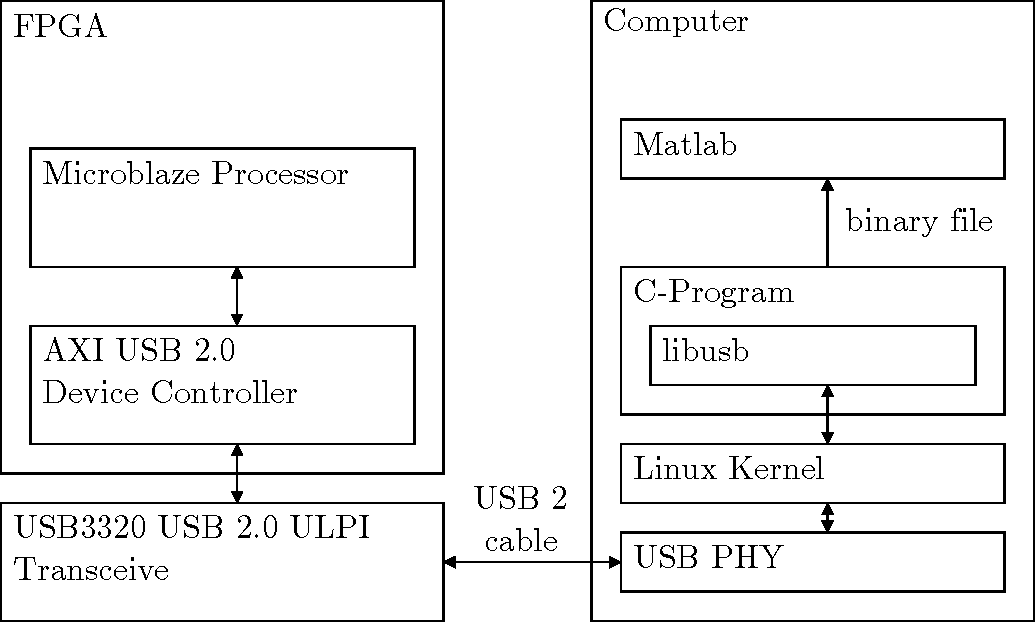
\includegraphics[width=0.6\textwidth]{figures/fpga_download}
  \caption{Overview of Download Process}
  \label{fig:fpga_download}
\end{figure}

\section{Clock domains}
\label{sec:fpga_clocks}

As a result of the different clocking constraints of the externals interfaces,
a relatively complex clocking scheme had to be applied as drawn in
\figref{fig:fpga_clock_domains}. Except for parts of the \gls{IO} interfaces,
synchronous positive edge triggered registers were used. For the synchronization
of the data paths crossing clock boundaries the numerous FIFO36E1 primitives
were used. Those configure the block \gls{RAM} cells to act as a \gls{FIFO}
memory. A wrapper is used to use many of those primitives to allow for the
wide vectors of up to 540 bits.
An exception are the \gls{ADC} and \gls{RAM} blocks which use
specialized \gls{INFIFO} and OUT\_FIFO and can do a 1:2 de-/multiplexing
using two independent input and output clocks. \\

\figref{fig:fpga_clock_generation} shows all the \glspl{PLL} used to derive the
different clocks. Because the \gls{MIG} core designed by Xilinx includes
it's own \gls{PLL} which optimally is directly connected to an external
clock source, the \gls{LVDS} signal of the SiT9102 200 MHz Fixed Frequency
Oscillator is directly connected to the \gls{PLL} inside the \gls{MIG} core.
The derived 125 MHz \gls{RAM} \gls{UI} clock is than used by the main
\gls{PLL} to derive all needed clocks for the peripheral. \\

In the following sections the clocking constraints of the different modules
are described. The closely related reset implementation is described
in \secref{sec:fpga_reset}. \\

\subsection{\gls{ADC}}
The \gls{ADC} provides a clock parallel to each of the four data streams.
The four clocks I0 Clk, I1 Clk, Q0 Clk and Q1 Clk are shown on
\figref{fig:fpga_architecture_overview} and are referred to as \gls{ADC} clocks.
They can be up to 900 MHz (1.8 $\text{GS}/\text{s}$ \gls{DDR})
and also significantly slower for slow (e.g. 800 $\text{MS}/\text{s}$)
sampling rates. \\

Each differential \gls{ADC} clock clock is first converted to a single ended
clock and than fed into a \gls{PLL} located next to the corresponding input
bank. This \gls{PLL} outputs a new clock in a local clock region
with the same frequency but an arbitrary phase shift
to clock the \gls{IDDR} and \gls{INFIFO} as described in \secref{sec:fpga_adc}.
Since the edges of the \gls{ADC} clocks and the corresponding data lines
are aligned, a phase shift of $90^\circ$ was found to work well and captures
the data during the stable period. \\

After parallelisation a new clock domain, the \gls{ADC} \gls{UI} clock
is used to do the centralization and reordering as described in
\secref{sec:fpga_adc_s3},
to do the bus conversion and finally to put the data into a \gls{FIFO}
traversing to the clock region of the \gls{RAM} \gls{UI} described
in \secref{sec:fpga_storage}. This clock has to be strictly greater than
$\frac{900\;\text{MHz}}{4} = 225\;\text{MHz}$ to avoid the
\gls{INFIFO} from filling up. Also there needs to be a minimal
distance between an edge of the \gls{ADC} \gls{UI} and the
\gls{RAM} \gls{UI} clock in order for the FIFO36E1 to work correctly.
Hence a clock rate of 250 MHz was chosen. \\

\subsection{\gls{RAM}}
\label{sec:fpga_clock_ram}
The used \gls{DDR} \gls{RAM} module can be clocked up to 800 MHz which would
allow for a data rate of
$2 \cdot 64\;\text{bit} \cdot 800\;\text{MHz} = 12.8 \text{GB} / \text{s}$.
As described in \secref{sec:fpga_storage}, a lower frequency of 500 MHz
was chosen. To allow interfacing the \gls{MB} at a as low as possible speed,
the \gls{MIG} core was configured to use an internal 1:4 multiplexing. This results
in \gls{RAM} \gls{UI} clock of 125 MHz.

\subsection{\acrfull{MB}}
Finally the \gls{MB} processor described in \secref{sec:fpga_download} has
it's own clock running at 100 MHz. \\

Later test runs showed, that the warning of the Platform studio saying that the
\gls{MB} runs only up to 100 MHz could be ignored and the \gls{MB} including
the \gls{USB} interface can run at 125 MHz as well. This removes one clock boundary
slightly increases the download speed by faster copying data from the
\gls{RAM} to the \gls{USB} buffer. \\

\begin{figure}
  \centering
  \includegraphics[width=0.7\textwidth]{figures/clock_generation}
  \caption{Block Diagram of Clock Generation}
  \label{fig:fpga_clock_generation}
\end{figure}

\begin{figure}
  \centering
  \includegraphics[width=\textwidth]{figures/fpga_clock_domains_overview}
  \caption{Overview of Clock Domains}
  \label{fig:fpga_clock_domains}
\end{figure}

\section{Resets}
\label{sec:fpga_reset}

In consequence of the many clocking regions, implementing a correct
reset scheme turned out to be trickier than one might think. \\

In general high active asynchronous resets were implemented for all
registers. Whenever a clock boundary had to be crossed, a reset synchronizer
as shown in \figref{fig:fpga_rst_sync} was used. The first register
makes sure the reset is release synchronous to the positive clock edge
of the target clock in order to have a full clock period to distribute
the reset signal so all target registers. The second register is
to make sure possible meta stability problems of the first registers would
no propagate. Clock and reset distribution networks both need to
distribute a signal with a limited amount of jitter and skew to a possibly
high fan-out. Therefor the same routing resources can be used.  \\

An overview of the reset distribution is given in
\figref{fig:fpga_rst_generation}. The reset can be triggered
by an external button or by the general reset of the \gls{FPGA}
used while downloading the bit file. Because the main system clock is
not available during reset, this reset input is debounced using a
156 MHz clock generated by a second oscillator on the VC707 board.
When the reset is released, first the \gls{MIG} core starts
it's \gls{PLL}, needs some time to initialize the \gls{RAM} and than
outputs a initialization complete signal which is used to derive the main reset
for the rest of the logic including the \gls{MB} and \gls{ADC} modules.
This main reset signal is than first synchronized to 5 MHz which is a
integer divider of all clocks and therefore is only released synchronous
to all clocks. \\

Because the very long setup time of the synchronous reset input of the FIFO36E1
can only be met at 240 MHz if there is a reset synchronization register
close to the FIFO primitive. Two 5 MHz synchronous global resets are than
globally distributed. The normal master reset used for all logic except
for the \glspl{FIFO}. They have an additional reset synchronizer, which is
placed next to each \gls{FIFO} primitive, prevented from being trimmed
away by logic optimization and has no output buffer.
This additional reset synchronizers are reset by the second global reset network
which releases the reset two 5 MHz clock periods earlier.  \\

Another challenge was to correctly reset the \gls{INFIFO} used in the
\gls{ADC} module as described in \secref{sec:fpga_adc}. These \glspl{FIFO}
cross the boundary between the clock regions provided by the \gls{ADC} and
the internal 250 MHz clock. The 4 clocks of the 4 channels might
have a slightly different phase, are derived from the same clock, the
\gls{ADC} sampling clock, though. It is crucial to release the reset
of all \gls{INFIFO} during the same \gls{ADC} sampling clock period to avoid
misalignment of the data. For that purpose, the global 5 MHz
reset is first synchronized to a phase shifted version of I0's clock and
than synchronized to the four \gls{ADC} clocks. \\

\begin{figure}
  \centering
  \includegraphics{figures/RstSync}
  \caption{Reset Synchronizer used to cross clock domains}
  \label{fig:fpga_rst_sync}
\end{figure}

\begin{figure}
  \centering
  \includegraphics[width=0.7\textwidth]{figures/rst_generation}
  \caption{Overview of the Reset Distribution}
  \label{fig:fpga_rst_generation}
\end{figure}

\section{Tools \& Development flow}
\label{sec:fpga_tools}

The \gls{FPGA} design and it's software consists of three different
main parts: \\

First the \gls{ADC} interface, the \gls{RAM} and the connecting
glue logic was implemented to be able store data sampled by the \gls{ADC}
in the \gls{RAM}. This part was fully developed using the Xilinx ISE 14.4
design suite. For testing an debugging manually inserted ChipScope
instruments were used, which form a logic analyzer running on the \gls{FPGA}
alongside the other modules. Since these instruments shares the same logic,
memory and routing resources, they heavily influence the mapping and routing
of the logic and therefor the timing of the circuit which can make debugging
timing problems cumbersome. \\
This project than interfaces directly to many externals pins and implements
the \gls{AXI} bus interface which was tied to dummy inputs for synthesis in ISE.
\\

In a second step, Xilinx Platform Studio, which is part of the Xilinx
\gls{EDK} 14.4, was used to create a project build around the \acrfull{MB}
soft-core processor. The ISE project consisting of the \gls{ADC} and \gls{RAM}
interface forms a peripheral. \\

In a third step, the software running on the \gls{MB} processor had to be
developed. This was done using Emacs and the Xilinx \gls{EDK} tools
consisting mainly of an Eclipse plugin. \\

The development process of course was not linear. These three steps were
iterated over multiple times. A complete run of synthesis, map,
place \& route, timing analysis and bit file generation
took between 20 minutes and 2 hours depending on how tight the timing was
and on how big the memory of the ChipScope instruments was chosen.
Since especially the debugging of the \gls{RAM} module and the implementation of
a correct reset behaviour (see \secref{sec:fpga_reset}) included a lot of
trial \& error, dozens of \gls{CPU} and man hours were spent on the
compiling the design.

%%  LocalWords:  FPGA Virtex VC Matlab DDR fpga Adc Microblaze AXI rf
%%  LocalWords:  AxiSlave Req Ack stallable req ack LUT virtex FMC ns
%%  LocalWords:  adc ASIC CMOS LVDS parallelised parallelise IBUFDS
%%  LocalWords:  parallelisation IDDR Xilinx MMCME MSB deasserted JTF
%%  LocalWords:  GiB MiB IP UI CP UART IC Mbit Tri PHY Gbit SGMII UDP
%%  LocalWords:  INetP ULPI FSM DMA middleware libusb de PLL SiT Clk
%%  LocalWords:  synchronizer rst jitter debounced synchronizers ISE
%%  LocalWords:  ChipScope EDK

\chapter{Characterization of Components and Equipment}
\label{chap:comp}

\section{R\&S Vector Network Analyzer ZNB8}
In order to gain a deeper understanding of the non-idealities of the
components which were later used for the different test setups
were characterized using a Rohde \& Schwarz Vector Network Analyzer. \\

Besides the results of the measurements of which a few a presented
in the next few sections, also important lessons about measuring were
learned. It took me about one week to be able to perform meaningful
measurements on the ZNB4 and to understand it's features.
While performing different measurements it soon became very clear then
non optimal torque while connection plugs or overbended cables
can produce notches of dozens of dBs even when using highest quality
equipment. \\
\begin{table}[h]
  \centering
  \begin{tabular}{|l|l|}
    \hline
    Frequency range & 9 kHz to 8.5 GHz \\ \hline
    Sweep speed & about 1ms for 100 points \\ \hline
    Dynamic range & up to 140 dB \\ \hline
    Power sweep range & 98 dB \\ \hline
  \end{tabular}
  \caption{Key properties of R\&S Vector Network Analyzer ZNB8}
  \label{tab:awg}
\end{table}

\section{Arbitrary waveform generator: Tektronix AWG 7122C}
\label{sec:comp_awg}
An \acrfull{AWG} was used instead of a real transmitter.
Not only because there is no transmitter available but also because of
it's flexibility. The same Matlab script used for simulations could
also call function output the baseband or the \gls{IF} signal.
The additional marker outputs could be used to trigger the oscilloscope
as well as the data acquisition process on the \gls{FPGA}.

\begin{table}[h]
  \centering
  \begin{tabular}{|l|l|}
    \hline
    Sample Rate & 12 $\text{GS}/\text{s}$, 24 $\text{GS}/\text{s}$ (interleaved) \\ \hline
    Number of analog channels & 2, 1 interleaved \\ \hline
    Analog bandwidth & 5.6 GHz \\ \hline
    Number of digital maker channels & $2 \times 2$ \\ \hline
    Vertical resolution & 8 Bit, 10 Bit when markers are disabled \\ \hline
    Maximal waveform length & 64 MS  \\ \hline
  \end{tabular}
  \caption{Key properties of Tektronix AWG 7122C}
  \label{tab:awg}
\end{table}

\section{Sivers IMA 58-63 GHz Converter FC1005V/00}
\label{sec:comp_sivers}
The most important is component in the transmission chain is the
up- and down-converter from an \acrfull{IF} to the \acrfull{RF}.
For this purpose the Sivers IMA FC1005V/00 module was used.
It consists of an independent transmit and receive path including
a horn antenna assembly, amplifiers, up-/down-mixers and a \gls{PLL}
for frequency synthesis. It is able up-/down-mix an \gls{IF}
of between 1 and 5 GHz to the \gls{RF} of 58 to 63 GHz. \\

As shown in \figref{fig:sivers} both the transmit and receive path
use two inputs (I- and Q-channel) which are then both mixed to
\gls{RF} and than fed to a $90^\circ$ hybrid coupler. \\
This results in one of the two mirror frequency to be completely canceled
if one channel is shifted by $-90^\circ$ relative to the other.
This can be done by using another $90^\circ$ hybrid coupler working on
\gls{IF} as described in \secref{sec:comp_90deg} or by using die Hilbert
transform as shown in \secref{sec:rx_rf_1}. \\
The Sivers module is build such that it transmits on the \gls{USBand}
(canceling the \gls{LSBand}) when the Q-channel is connected to the signal
$x(t)$ and the I-channel to $\mathcal{H}\{x(t)\}$. \\

There are two independent \gls{LO} for transmission and reception both using
the reference. There is an internal 10 MHz reference on the board. During
most measurements the reference was locked to same external reference as the
\gls{AWG} and \gls{ADC} to not have any frequency offsets when different
transmit and receive frequencies were used.

\begin{figure}[p]
  \centering
  \includegraphics[width=\textwidth]{pictures/sivers}
  \caption{Picture of Sivers IMA FC1005V/00 Converter}
  \label{fig:sivers}
\end{figure}

\begin{figure}[p]
  \centering
  \includegraphics[width=\textwidth]{figures/sivers_block_diagram}
  \caption{Block diagram of Sivers IMA FC1005V/00 Converter \cite{sivers_fc1005v}}
  \label{fig:sivers}
\end{figure}

\begin{table}
  \centering
  \begin{tabular}{|l|l|}
    \hline
    \gls{TX} and \gls{RX} \gls{RF} range & 58 - 63 GHz \\ \hline
    \gls{TX} and \gls{RX} \gls{IF} range & 1 - 5 GHz \\ \hline
    Saturated output power & min 16 dBm \\ \hline
    \gls{LO} leakage & typical 10 dBm, max 15 dBm \\ \hline
    \gls{TX} Image rejection & min 10 dB, typical 20 dB \\ \hline
    \gls{RX} Image rejection & min 10 dB, typical 14 dB \\ \hline
    Total Power Consumption & 9.5 W \\ \hline
    1-dB output compression point & 10 dBm \\ \hline
    Nominal gain \gls{IF} to \gls{RF} & 25 - 40 db \\ \hline
  \end{tabular}
  \caption{Key properties of 58-63 GHz V-band Converter Sivers IMA FC1005V/00
    \cite{sivers_fc1005v}}
  \label{tab:awg}
\end{table}

\section{Meca 3 dB Hybrid Coupler 705S-3.000}
\label{sec:comp_90deg}

A Hybrid coupler has typically 4 ports as shown on
\figref{fig:90deg_coupler_symbol}.
One port is often 50 $\Omega$ terminated and therefor might not be connected
to a plug. \\

It is, when neglecting production imperfections, a fully symmetric component
(inputs $x_i(t)$ with outputs $y_i(t)$ as well as indices 1 and 2
can be exchanged) and has the following relations:

\begin{align}
  y_1(t) = \frac{1}{\sqrt{2}} \left[x_1(t) \angle -\frac{\pi}{2} + x_2(t) \angle -\pi \right] \\
  y_2(t) = \frac{1}{\sqrt{2}} \left[x_1(t) \angle -\pi + x_2(t) \angle -\frac{\pi}{2} \right]
\end{align}

As shown in \figref{fig:90deg_coupler_measurement} the power of
$x_1$ is not perfect equally split to $y_1$ and $y_2$. The power difference
is smaller than 1 db in the band from 1.8 GHz to 4 GHz.
Also there is a little power ($\leq -20 db$) leaking from $x_1$ to $x_2$ and from
$y_1$ to $y_2$. \\

Due to missing calibration equipment the phase rotation could not be measured.
All measured numbers matched the specifications.

\begin{figure}[p]
  \centering
  \includegraphics{figures/90deg_coupler_symbol}
  \caption{Symbol of a $90^\circ$ Coupler}
  \label{fig:90deg_coupler_symbol}
\end{figure}

\begin{figure}[p]
  \centering
  \includegraphics[width=\textwidth]{figures/network_analyzer/Meca_705S-3_coupler_id1}
  \caption{Measurements of Meca 3 dB Hybrid Coupler 705S-3.000,
    $x_1 \triangleq $ port 1, $y_1 \triangleq $ = port 2,
    $x_2 \triangleq $ port 3, $y_2 \triangleq $ = port 4}
  \label{fig:90deg_coupler_measurement}
\end{figure}

\begin{table}[h]
  \centering
  \begin{tabular}{|l|l|}
    \hline
    Operation range & 2 - 4 GHz \\ \hline
    Frequency Sensitivity & $\pm$ 0.4 dB \\ \hline
    Coupling variation & 3.1 dB $\pm$ 0.6 db \\ \hline
    Typical Isolation & 22 dB \\ \hline
    max \gls{VSWR} & 1.2 : 1 \\ \hline
    Phase rotation & $90^\circ \pm 2.0^\circ$ \\ \hline
  \end{tabular}
  \caption{Key properties of Meca 3 dB Hybrid Coupler 705S-3.000 \cite{meca_705s}}
  \label{tab:awg}
\end{table}

\section{Mini-Circuits Amplifier ZX60-V63+}
Whenever additional gain was needed to drive a mixer input or the \gls{ADC}
with the proper power level, power amplifiers made by Mini-Circuits were used. \\

It's key properties are shown in \tblref{tab:comp_zx60}, a picture is shown in
\figref{fig:comp_zx60_pic} and my own gain and \gls{VSWR} measurements are shown in
\figref{fig:comp_zx60_meas}. \\

\begin{table}
  \centering
  \begin{tabular}{|l|l|}
    \hline
    Operation range & 0.05 - 6 GHz \\ \hline
    Gain & 21.9 dB typ. at 0.05 GHz, 15.4 dB typ. at 6 GHz \\ \hline
    Flatness & $\pm$ 1.7 dB from 50 to 3000 MHz \\ \hline
    1 dB compression point (out. power) & min. 17 dBm \\ \hline
  \end{tabular}
  \caption{Key properties of Mini-Circuits Amplifier ZX60-V63+ \cite{mc_zx60}}
  \label{tab:comp_zx60}
\end{table}

\begin{figure}[p]
  \centering
  \includegraphics[width=0.4\textwidth]{pictures/ZX60-V63+}
  \caption{\gls{MC} Amplifier ZX60-V63+}
  \label{fig:comp_zx60_pic}
\end{figure}

\begin{figure}[p]
  \centering
  \begin{subfigure}{0.45\textwidth}
    \centering
    \includegraphics[width=\textwidth]{figures/network_analyzer/MCL_ZX60-V63+_Amplifier_S11_id1}
    \caption{\gls{VSWR} of the input}
  \end{subfigure}
  ~
  \begin{subfigure}{0.45\textwidth}
    \centering
    \includegraphics[width=\textwidth]{figures/network_analyzer/MCL_ZX60-V63+_Amplifier_S21_id1}
    \caption{Gain vs. Frequency}
  \end{subfigure}
  \caption{Measurements of Mini-Circuits Amplifier ZX60-V63+,
    input $\triangleq$ port 1, output $\triangleq$ port 2}
  \label{fig:comp_zx60_meas}
\end{figure}

\section{Mini-Circuits High-pass Filter BHP-1000+}
For the setup described in \chapref{chap:res_450}, a high-pass filter
by Mini-Circuits was as the lower bound for the channel selection filter.
It's properties are listed in \tblref{tab:comp_bhp1000} and a picture is given in
\figref{fig:comp_bhp1000_pic}.

\begin{table}
  \centering
  \begin{tabular}{|l|l|}
    \hline
    Stop Band ($\geq$3dB) & $<$ 0.9 GHz \\ \hline
    Pass Band ($<$ 1dB) & 1 - 3 GHz \\ \hline
  \end{tabular}
  \caption{Key properties of High-pass Filter BHP-1000+ \cite{mc_bhp1000}}
  \label{tab:comp_zx60}
\end{table}

\begin{figure}[p]
  \centering
  \includegraphics[width=0.4\textwidth]{pictures/BHP-1000+}
  \caption{High-pass Filter BHP-1000+}
  \label{fig:comp_bhp1000_pic}
\end{figure}

\section{Mini-Circuits DC Block MCL BLK-89-S+}
\label{sec:comp_dc_block}
To prevent \gls{DC} from driving amplifier inputs into saturation
a \gls{DC}-block was used. A significantly higher insertion loss was
measured than specified in the data sheet as shown in
\tblref{tab:comp_dc_block} and \figref{fig:comp_dc_block_insertion_loss}.

\begin{table}[h]
  \centering
  \begin{tabular}{|l|l|}
    \hline
    Pass Band & 0.1 MHz to 8 GHz \\ \hline
    Specified Insertion loss up to 4 GHz & $<$ 0.8 dB \\ \hline
    Measured Insertion loss up to 4 GHz & $<$ 0.8 dB \\ \hline
  \end{tabular}
  \caption{Key properties of Mini-Circuits DC Block MCL BLK-89-S+ \cite{mc_blk89}}
  \label{tab:comp_dc_block}
\end{table}

\begin{figure}[p]
  \centering
  \includegraphics[width=\textwidth]{figures/network_analyzer/MCL_BLK-89-S+_DC-Block_insertion_loss}
  \caption{Measured Insertion Loss of Mini-Circuits DC Block MCL BLK-89-S+}
  \label{fig:comp_dc_block_insertion_loss}
\end{figure}

\section{Mini-Circuits Attenuators VAT+}
\label{sec:comp_vat}
To adjust all the power levels across the \gls{RF} part, fixed
attenuators were used. The 1 dB version is shown in
\figref{fig:comp_vat_pic}. \tblref{tab:comp_vat} shown the key properties
of these attenuators.

\begin{table}[h]
  \centering
  \begin{tabular}{|l|l|}
    \hline
    Operation range & DC - 6 GHz \\ \hline
  \end{tabular}
  \caption{Key property of Mini-Circuits Attenuators VAT+ \cite{mc_vat1}}
  \label{tab:comp_dc_block}
\end{table}

\begin{figure}[p]
  \centering
  \includegraphics[width=0.4\textwidth]{pictures/attenuator}
  \caption{\gls{MC} attenuators}
  \label{fig:comp_vat_pic}
\end{figure}

\section{Texas-Instruments Baluns ADC-WB-BB and ADC-LB-BB}
\label{sec:comp_balun}
The received \gls{IF} signals are single ended and the impedance of all
components and cables is 50 $\Omega$. The \gls{ADC} on the other hand, uses
differential inputs with an impedance of 100 $\Omega$. Therefor baluns are used
for conversion. The \gls{VSWR} and insertion loss measurements of the used
ADC-WB-BB are shown in \figref{fig:comp_wbbb}. The ADC-LB-BB, which was also
available was not used due to it's high insertion loss at low frequencies. \\

\begin{figure}[p]
  \centering
  \begin{subfigure}{0.45\textwidth}
    \centering
    \includegraphics[width=\textwidth]{figures/network_analyzer/TI_ADC-WB-BB_Balun_swr_id1}
    \caption{\gls{VSWR} of the input}
  \end{subfigure}
  ~
  \begin{subfigure}{0.45\textwidth}
    \centering
    \includegraphics[width=\textwidth]{figures/network_analyzer/TI_ADC-WB-BB_Balun_insertion_loss_id1}
    \caption{Insertion Loss}
  \end{subfigure}
  \caption{Measurements of Texas-Instruments Balun ADC-WB-BB,
    input $\triangleq$ port 1, output $\triangleq$ port 2}
  \label{fig:comp_wbbb}
\end{figure}

\begin{figure}[p]
  \centering
  \begin{subfigure}{0.45\textwidth}
    \centering
    \includegraphics[width=\textwidth]{figures/network_analyzer/TI_ADC-LB-BB_Balun_swr_id1}
    \caption{\gls{VSWR} of the input}
  \end{subfigure}
  ~
  \begin{subfigure}{0.45\textwidth}
    \centering
    \includegraphics[width=\textwidth]{figures/network_analyzer/TI_ADC-LB-BB_Balun_insertion_loss_id1}
    \caption{Insertion Loss}
  \end{subfigure}
  \caption{Measurements of Texas-Instruments Balun ADC-LB-BB,
    input $\triangleq$ port 1, output $\triangleq$ port 2}
  \label{fig:comp_lbbb}
\end{figure}

\begin{figure}[p]
  \centering
  %\includegraphics[width=0.4\textwidth]{pictures/}
  \caption{Picture of Texas-Instruments Balun ADC-WB-BB}
  \label{fig:comp_balun_pic}
\end{figure}

\section{Texas Instruments ADC 12d1800}
\label{sec:comp_adc}
The receiver was build using the Ultra High-Speed ADC12D1800 by Texas Instruments.
It is able to either sample two channels at 1.8 $\text{GS}/\text{s}$ or to interleave
this two channels by applying the same input signal to both channels and sampling
one on the positive and the other one on the negative clock edge resulting in sample
rates of up to 3.6 $\text{GS}/\text{s}$. The vertical resolution of 12 bits is better
than the one of the used oscilloscope (\secref{sec:comp_osci}) and in most scenarios
not the \gls{SNR} limiting factor even when the signal is 6 db below full-scale.
The huge analog bandwidth of about 100 kHz
(limited by the \gls{DC} block described in \secref{sec:comp_dc_block}) to about
2.8 GHz allows to not only sample the first Nyquist-zone but also allows
for sub-sampling which was particular interest. \\

The ADC12D1800 Reference Board was used which has a very well optimized board
layout, supports \gls{SMA} plugs for all important signals, includes a
\gls{FPGA} and \gls{USB} interface for configuration and a power supply.
The reference board has an on-board \gls{PLL} but was often clocked by a marker
output of the \gls{AWG}.
An \gls{FMC} connector exposes the full interface of the \gls{ADC} to
the on board \gls{FPGA} and is used by the Virtex-7 board to capture the data
as described in \chapref{chap:fpga}. \\

\begin{table}[h]
  \centering
  \begin{tabular}{|l|l|}
    \hline
    Number of channels & 2, 1 interleaved \\ \hline
    Sample Rate & $\leq$ 1.8 $\text{GS}/\text{s}$, $\leq$ 3.6 $\text{GS}/\text{s}$ interleaved \\ \hline
    Analog Bandwidth & typical 2.8 GHz \\ \hline
    Vertical Resolution & 12 bit \\ \hline
    Noise Floor Density & $\approx$ -150 $\text{dB}/\text{Hz}$ \\ \hline
    Power Consumption & 4.7 W \\ \hline
  \end{tabular}
  \caption{Key properties of Texas-Instruments ADC 12d1800 \cite{ti_adc12d1800}}
  \label{tab:comp_adc}
\end{table}

\section{Xilinx Virtex 7 Board VC707}
\label{sec:comp_vc707}
For the data acquisition and storage the VC707 Virtex-7 evaluation board
was used. It's key features are listed in \tblref{tab:comp_vc707} and a
picture is shown in \figref{fig:comp_vc707_pic}.


\begin{table}[h]
  \centering
  \begin{tabular}{|l|l|}
    \hline
    Bit-File Storage & 128 MB Linear byte peripheral interface (BPI) Flash memory \\ \hline
    Download-Interface & USB 2.0 ULPI Transceiver \\ \hline
    Program \& Debug Interface & USB JTAG through Digilent module \\ \hline
    User I/O & 5 Push-Buttons, 4 GPIO SMA plugs \\ \hline
    Connection to \gls{ADC} board & VITA 57.1 FMC1 HPC Connector \\ \hline
    Logic Cells & 85'760 \\ \hline
    Block RAM Size &  37'080 kB \\ \hline
    Total I/O Banks & 14 \\ \hline
  \end{tabular}
  \caption{Relevant properties of Xilinx Virtex 7 Evaluation Board VC707
    \cite{xilinx_virtex7_overview, xilinx_vc707}}
  \label{tab:comp_vc707}
\end{table}

\begin{figure}[p]
  \centering
  \includegraphics[width=\textwidth]{pictures/vc707}
  \caption{Picture of Xilinx Virtex 7 Evaluation Board VC707}
  \label{fig:comp_vc707_pic}
\end{figure}

\section{R\&S Oscilloscope RTO 1044}
\label{sec:comp_osci}
High frequency measurements were made on a Rohde \& Schwarz Digital
Oscilloscope RTO 1044. With the optional reference input it could be locked
to the \gls{AWG} as well used to have a very precise ($\pm 0.02 \text{ppm}$),
oven controlled 10 MHz reference. \\

During many experiments the real time \gls{FFT} display of the oscilloscope was
proven very useful to check power levels and signal shapes. \\

Since the VISA standard for instrument control is painful to install under
Redhat 6 a small program based on the VXI-11 library written by
Steve D. Sharples\footnote{see: http://optics.eee.nottingham.ac.uk/vxi11/}
was written to convert simple telnet commands send by Matlab
to remote procedure calls. This allowed to setup and readout the oscilloscope
directly in the Matlab simulation framework. This was used to do first experiments
on the actual \gls{RF} hardware before the \gls{FPGA} (\chapref{chap:fpga}) was
completely implemented. \\

\begin{table}[h]
  \centering
  \begin{tabular}{|l|l|}
    \hline
    Number of channels & 4, 2 interleaved \\ \hline
    Sample Rate & 10 $\text{GS}/\text{s}$, 20 $\text{GS}/\text{s}$ interleaved \\ \hline
    Analog Bandwidth at 50 $\Omega$ & $\geq 4$ GHz \\ \hline
    Vertical Resolution & 8 bit \\ \hline
  \end{tabular}
  \caption{Key properties of R\&S Oscilloscope RTO 1044}
  \label{tab:awg}
\end{table}

%%  LocalWords:  datasheets ZNB idealities Rohde Schwarz overbended
%%  LocalWords:  dBs Tektronix AWG Matlab baseband FPGA Sivers IMA FC
%%  LocalWords:  PLL sivers coupler USBand LSBand LSB ima dBm Meca WB
%%  LocalWords:  VSWR Balun MCL BLK osci SNR Nyquist SMA FMC Virtex
%%  LocalWords:  fpga Xilinx VC RTO FFT Redhat VXI Sharples rx rf ZX
%%  LocalWords:  zx typ BHP bhp Attenuators attenuators Baluns baluns
%%  LocalWords:  wbbb vc BPI ULPI JTAG Digilent GPIO HPC kB

\chapter{Measurements}
\section{Narrow Band Transmission}
\label{sec:res_450}

First a relatively narrow signal transmitting at only a quarter
of the maximal symbol rate was build and analyzed to show some basic
properties of the system and to show what the best achievable
\gls{EVM} values are. \\

As receiver architecture, the Quadrature Intermediate Frequency Sub-Nyquist
Sampling Receiver as described in \secref{sec:rx_2} is used with the difference
that the signal bandwith is only $B = 450 MHz$. All the other properties are listed
in \tblref{tab:res_450}. \\

\begin{table}[h]
  \centering
  \begin{tabular}{|l|r@{}l@{~}l|}
    \hline
    $f_{\text{TX IF}}$ & 2&.9&GHz \\ \hline
    $f_{\text{TX LO}}$ & 57&.5&GHz \\ \hline
    $f_{\text{RX LO}}$ & 58&.2&GHz \\ \hline
    $f_{\text{RX IF}}$ & 2&.2&GHz \\ \hline
    $f_c$            & 60&.4&GHz \\ \hline
    Signal Bandwidth B & 0&.45&GHz \\ \hline
    Sample Rate $f_s$ & 1&.8&GHz \\ \hline
  \end{tabular}
  \caption{Properties of Narrow Band Transmission System}
  \label{tab:res_450}
\end{table}

\subsection{Measurement Setup and RF System Analysis}
A block diagram providing an overview of the test setup,
used for all following measurements, can be found in \figref{fig:res_450_bd}. \\

\begin{figure}[p]
  \centering
  %\includegraphics[width=\textwidth]{pictures/res_450_setup}
  \caption{Block Diagram of the Narrow Band Transmission Setup}
  \label{fig:res_450_bd}
\end{figure}
\todo{draw block diagram}

\begin{figure}[p]
  \centering
  \includegraphics[width=\textwidth]{pictures/res_450_setup}
  \caption{Picture of the Narrow Band Transmission Setup}
  \label{fig:res_450_pic}
\end{figure}

\subsubsection{Matlab}
The Matlab script was configured such that it generates the transmitt signal,
programs the \gls{AWG}, reads the data acquired by the \gls{FPGA},
runs the receiver code and finally generets reports and figures. \\
The configuration file used for these tests can be found in
\appref{app:res_450_cnf}. \\

\subsubsection{\gls{AWG}}
The \gls{AWG} was configured to output the \gls{TX} \gls{IF} signal $i[k]$,
the sample clock for the \gls{ADC} as well as synchronization pulses to trigger
the \gls{FPGA} and oscillocope. It's configuration and port assignment
are shown in \tblref{tab:res_450_awg}.

It was noticed, that the used \gls{AWG} has some cross talk from
channel 1 marker 1 output to the channel 1 analog output. Therefor the
\gls{ADC} clock should always be output on marker 2 and not on marker 1.
For synchronization pulses, this is not an issue, since they are ware always
configured to give a 100 cycle wide positive pulse $> 100 \text{ns}$ before
the signal starts. \\

\begin{table}[h]
  \centering
  \begin{tabular}{|l|l|}
    \hline
    Sampling Rate & 10.8 GS/s \\ \hline
    Clock Source & Externals 10 MHz \\ \hline
    Analog Amplitude & 1 $\text{V}_{\text{pp}}$ \\ \hline
    Marker Amplitude CH1 Marker 1/2 & 0, 0.7 V \\ \hline
    Marker Amplitude CH2 Marker 1/2 & 0, 1.4 V \\ \hline
    \gls{DAC} resolution & 8 bit \\ \hline
    CH 1 & $i[k]$ \\ \hline
    CH 2 & $\mathcal{H}\{i[k]\}$ \\ \hline
    CH 1 Marker 1 & 0 \\ \hline
    CH 1 Marker 2 & 1.8 GHz \gls{ADC} sample clock \\ \hline
    CH 2 Marker 1 / 2 & Sync pulse before frame starts \\ \hline
  \end{tabular}
  \caption{Configuration and Port Assignment of \gls{AWG}}
  \label{tab:res_450}
\end{table}

An osilloscope plot (see \secref{sec:comp_osci}) of the generated
\gls{TX} \gls{IF} signal and it's \gls{FFT} can be found in
\figref{fig:res_450_awg_analog}.
The \gls{ADC} clock signal and the sync pulse are shown
in \figref{fig:res_450_awg_digital}. \\

\begin{figure}[p]
  \centering
  \includegraphics[width=\textwidth]{figures/osci/res_450_awg_analog}
  \caption{\gls{TX} \gls{IF} signal generated by the \gls{AWG}}
  \label{fig:res_450_awg_analog}
\end{figure}

\begin{figure}[p]
  \centering
  \includegraphics[width=\textwidth]{figures/osci/res_450_awg_digital}
  \caption{\gls{ADC} clock signal and sync pulse generated by the \gls{AWG}}
  \label{fig:res_450_awg_digital}
\end{figure}

\subsubsection{RF parts}
The two analog channels generated by the \gls{AWG} have a total signal
power of -9.28 dBm each \eqref{eq:res_450_awg_pwr}. These signals were
than attenuated by 20 dB to be below the 1-dB output compression point of 10 dBm
of the 60 GHz converters even at full gain of 40 dB. \\

\begin{align}
  10 \cdot \log_{10}\left(
  10^{-25.812 \;\text{dBm} / 10} \cdot
  \frac{450 \;\text{MHz}}{10 \;\text{MHz}}
  \right) \approx -9.28 \;\;\text{dBm}
  \label{eq:res_450_awg_pwr}
\end{align}

The same 60 GHz converter was used for transmission and reception and
configured as shown in \tblref{tab:res_450_sivers} (configuration script
see \appref{app:}).
A 10 MHz reference clock was fed from the \gls{AWG}.
An aluminium plate in a distance of about 15 cm was used as a reflector. \\

\begin{table}[h]
  \centering
  \begin{tabular}{|l|l|}
    \hline
    Reference Clock & external \\ \hline
    TX Oscillator Frequency & 57.5 GHz (0x038170) \\ \hline
    RX Oscillator Frequency & 58.2 GHz (0x038D60) \\ \hline
    TX Power & 0x80 \\ \hline
  \end{tabular}
  \caption{Configuration Parameters of 60 GHz Converter}
  \label{tab:res_450}
\end{table}

Both channels on the \gls{RX} side of the converer first connect to a
\gls{MC} BHP-1000+ high-pass filter. As we can see in \figref{fig:res_450_rx_if},
the \gls{TX} \gls{LO} leackage is attenuated by about 35 dB. Also the \gls{TX}
\gls{LSBand} signal (centered around 3.6 GHz) is about 17 dB weaker than
the desired \gls{TX} \gls{USBand} signal. This is due to the transmitter's
image rejection and the fact that the \gls{LSBand} signal is outside the
\gls{RF} specification of the converter. \\

\begin{figure}[p]
  \centering
  \includegraphics[width=\textwidth]{figures/osci/res_450_rx_if}
  \caption{Received \gls{IF} Signal before (left) and after (right) High-Pass Filter}
  \label{fig:res_450_rx_if}
\end{figure}p

Next the signal amplified by 12 dB to drive the \gls{ADC} input to about 70\%
as shown in \figref{fig:res_450_rx_amp}. \\

\begin{figure}[p]
  \centering
  \includegraphics[width=\textwidth]{figures/osci/res_450_rx_amp}
  \caption{Received \gls{IF} Signal before (left) and after (right) the Amplifier}
  \label{fig:res_450_rx_amp}
\end{figure}

Finally the signal is converted to a differential signal using a ADC-WB-BB Balun
(\secref{sec:comp_balun}), passes a \gls{DC} block (\secref{sec:comp_dc_block})
and digitized by the \gls{ADC}. \\

The channel filter shown in \figref{fig:rx_2_bd} is therefor build using
the BHP-1000+ high-pass filter and the \gls{ADC} analog input bandwidth which
cuts of at about 2.8 GHz. \\

\subsection{Channel impulse response}
\label{sec:res_450_h}
First we should have a short look at the channel response of the simple
reflector. The estimated channel response using the Goaly estimator and a
1152 long \gls{CES} field is shown in \figref{fig:res_450_h}.
As we can see, there is one very distinctive peak confirming one single,
more or less flat, reflector. \\

\begin{figure}[p]
  \centering
  \includegraphics[width=0.8\textwidth]{figures/matlab/res_450_h}
  \caption{One realization of a measured channel impulse response in Time Domain
    with Narrow Band Transmission Setup}
  \label{fig:res_450_h}
\end{figure}

\subsubsection{Root Mean Square Delay Spread}
\begin{align}
  \overline{\tau} &=\frac{\int_0^\infty\tau A_c(\tau)d\tau}{\int_0^\infty A_c(\tau)d\tau} \\
  \tau_{\text{rms}} &=\sqrt{\frac{\int_0^\infty(\tau-\overline{\tau})^2
      A_c(\tau)d\tau}{\int_0^\infty A_c(\tau)d\tau}}
\end{align}

\subsubsection{Delay Spread}
Root Mean Square Delay Spread is a nice statistical property of a channel.
When designing a receiver, it is more relevant though, that we now how many
samples have to be considered to capture enough energy of a symbol. \\

How much energy is significant, can be estimated depending on the \gls{SNR}
we want to achiev. The \gls{SNR} we want to reach depends on the modulation rate
we want to achiev. Therefor we first calculate the needed \gls{SNR} for
\gls{QAM}-256. \\

\todo{do SNR calculation and calc delay spread}
The delay spread $\approx $ 5 ps, which corresponds to about 7 symbols
at 450 MS/s and about 15 symbols at 1.8 GS/s. \\

% EVM_D measurement 1 frame
% EVM_R measurement 1 frame
% -> inital rotation
% EVM_D rotation, increasing frame window
% -> worse, worse
% phase noise correction
% -> steady at EVM_R?

\subsection{Error Vector Magnitude Measurements}
\begin{figure}[p]
  \centering
  \includegraphics[width=0.6\textwidth]{figures/matlab/res_450_cp_synced}
  \caption{Received Data Points after Synchronization but before any Correction}
  \label{fig:res_450_cp_synced}
\end{figure}

\begin{figure}[p]
  \centering
  \includegraphics[width=0.6\textwidth]{figures/matlab/res_450_cp_corrected}
  \caption{Received Data Points after Correction (one color per data packet)}
  \label{fig:res_450_cp_corrected}
\end{figure}

As we can see in \figref{fig:res_450_cp_corrected} the pattern looks quite good,
after the channel and phase noise correction.
The whole pattern is rotated though, which leads to a bit error rate of
about 0.25. \\

Two different calculation schemes for the \acrfull{EVM} are used as described in
the following sections. \tblref{tab:res_450_evm} shown an overview of the
\gls{EVM} values.

\begin{table}[h]
  \centering
  \begin{tabular}{|l|l|}
    \hline
    $\text{EVM}_\text{D}$                           & ? \\ \hline
    $\text{EVM}_\text{R}$                           & ? \\ \hline
  \end{tabular}
  \caption{Measured \gls{EVM} values of the Narrow Band Transmission Experiment}
  \label{tab:res_450_evm}
\end{table}

\subsubsection{\acrfull{DEVM}}
The \gls{DEVM} is calculated as stated in \eqref{eq:devm} \cite{razavi2011rf}.

\begin{align}
  \text{EVM}_\text{D} &= \frac{1}{P_{\text{avg}}} \cdot \frac{1}{N}
  \sum_{j=0}^{N-1} |i_j - s_j|^2
  \label{eq:devm} \\
  \text{EVM}_\text{D}\text{dB} &= 10 \cdot \log_{10} (\text{EVM}_\text{D})
\end{align}

Where $N$ is the total number of symbols, $s_j$ the complex value of the
received symobol $j$ and $i_j$ the ideal position of the symbol. \\

\subsubsection{\acrfull{REVM}}
As we can see, the very bad \gls{DEVM} measured for the constellation in
\figref{fig:res_450_cp_corrected} is due to a deterministic error wihch will
be discuessed further in \secref{sec:res_450_phase}.

In order to get an figure of merit, which is not influenced, by those deterministic
errors, a slight adaption of the classical \gls{DEVM} definition was made. \\

The proposed \acrfull{REVM} builds one subset of the set of received points for
each available data symbol. The error vector $e_j$ is than calculated as the
difference of the received point and the mean of all received points of that
set. Therefor it does not matter, if all points corresponding to one sent symbol
are off. Instead we have a figure of merit telling, how far one sent symbol gets
spread. \\

\subsection{Phase Noise}
\label{sec:res_450_phase}

As we can see in \figref{}, where the phase of

\begin{itemize}
\item Phase-Noise plot measured using many short frames, show that correction algorithm works
\end{itemize}

\subsection{High Modulation Rate}
\begin{itemize}
\item Show that high modulation rates and multi GB/s throughput is possible (\gls{QAM} 256?)
\end{itemize}

\section{Full Bandwidth Transmission}
\subsection{Transmitter Channel Imbalance}
\begin{itemize}
\item Show that transmitter channel imbalance is not an issue
\end{itemize}

\subsection{90deg Coupler Error Measurement and Correction}
\begin{itemize}
\item Show error introduced by non-perfect 90 deg coupler.
\item Show the best correction I will come up with
\item Compare to best result achieved by classical architecture (with additional mixer)
\end{itemize}

%%  LocalWords:  multi QAM Coupler coupler

\chapter{Conclusion \& Outlook}
\begin{itemize}
\item Multi GB/s throughput is possible using high QAM modulation rates.
\item Phase noise must be considered.
\item Floating point Matlab implementations could be replaced by fixed-point implementations
\item Complete receiver could be implemented in FPGA
\end{itemize}

\begin{appendix}
  \chapter{ADC to FPGA connections}
\label{app:app_adc_fpga_con}
\begin{verbatim}
NET "ID1ClkPxCI"   LOC = "L31" |IOSTANDARD = LVDS; # bank=34, byte_group=1
NET "ID1ClkNxCI"   LOC = "K32" |IOSTANDARD = LVDS; # bank=34, byte_group=1
NET "ID1PxDI[0]"   LOC = "M32" |IOSTANDARD = LVDS; # bank=34, byte_group=1
NET "ID1NxDI[0]"   LOC = "L32" |IOSTANDARD = LVDS; # bank=34, byte_group=1
NET "ID1PxDI[1]"   LOC = "W30" |IOSTANDARD = LVDS; # bank=34, byte_group=3
NET "ID1NxDI[1]"   LOC = "W31" |IOSTANDARD = LVDS; # bank=34, byte_group=3
NET "ID1PxDI[2]"   LOC = "Y29" |IOSTANDARD = LVDS; # bank=34, byte_group=3
NET "ID1NxDI[2]"   LOC = "Y30" |IOSTANDARD = LVDS; # bank=34, byte_group=3
NET "ID1PxDI[3]"   LOC = "N28" |IOSTANDARD = LVDS; # bank=34, byte_group=2
NET "ID1NxDI[3]"   LOC = "N29" |IOSTANDARD = LVDS; # bank=34, byte_group=2
NET "ID1PxDI[4]"   LOC = "R28" |IOSTANDARD = LVDS; # bank=34, byte_group=2
NET "ID1NxDI[4]"   LOC = "P28" |IOSTANDARD = LVDS; # bank=34, byte_group=2
NET "ID1PxDI[5]"   LOC = "P30" |IOSTANDARD = LVDS; # bank=34, byte_group=2
NET "ID1NxDI[5]"   LOC = "N31" |IOSTANDARD = LVDS; # bank=34, byte_group=2
NET "ID1PxDI[6]"   LOC = "R30" |IOSTANDARD = LVDS; # bank=34, byte_group=2
NET "ID1NxDI[6]"   LOC = "P31" |IOSTANDARD = LVDS; # bank=34, byte_group=2
NET "ID1PxDI[7]"   LOC = "K29" |IOSTANDARD = LVDS; # bank=34, byte_group=1
NET "ID1NxDI[7]"   LOC = "K30" |IOSTANDARD = LVDS; # bank=34, byte_group=1
NET "ID1PxDI[8]"   LOC = "J30" |IOSTANDARD = LVDS; # bank=34, byte_group=1
NET "ID1NxDI[8]"   LOC = "H30" |IOSTANDARD = LVDS; # bank=34, byte_group=1
NET "ID1PxDI[9]"   LOC = "J31" |IOSTANDARD = LVDS; # bank=34, byte_group=1
NET "ID1NxDI[9]"   LOC = "H31" |IOSTANDARD = LVDS; # bank=34, byte_group=1
NET "ID1PxDI[10]"  LOC = "L29" |IOSTANDARD = LVDS; # bank=34, byte_group=1
NET "ID1NxDI[10]"  LOC = "L30" |IOSTANDARD = LVDS; # bank=34, byte_group=1
NET "ID1PxDI[11]"  LOC = "T29" |IOSTANDARD = LVDS; # bank=34, byte_group=3
NET "ID1NxDI[11]"  LOC = "T30" |IOSTANDARD = LVDS; # bank=34, byte_group=3
NET "ID0ClkPxCI"   LOC = "K39" |IOSTANDARD = LVDS; # bank=19, byte_group=1
NET "ID0ClkNxCI"   LOC = "K40" |IOSTANDARD = LVDS; # bank=19, byte_group=1
NET "ID0PxDI[0]"   LOC = "J40" |IOSTANDARD = LVDS; # bank=19, byte_group=1
NET "ID0NxDI[0]"   LOC = "J41" |IOSTANDARD = LVDS; # bank=19, byte_group=1
NET "ID0PxDI[1]"   LOC = "P41" |IOSTANDARD = LVDS; # bank=19, byte_group=3
NET "ID0NxDI[1]"   LOC = "N41" |IOSTANDARD = LVDS; # bank=19, byte_group=3
NET "ID0PxDI[2]"   LOC = "M42" |IOSTANDARD = LVDS; # bank=19, byte_group=2
NET "ID0NxDI[2]"   LOC = "L42" |IOSTANDARD = LVDS; # bank=19, byte_group=2
NET "ID0PxDI[3]"   LOC = "H40" |IOSTANDARD = LVDS; # bank=19, byte_group=1
NET "ID0NxDI[3]"   LOC = "H41" |IOSTANDARD = LVDS; # bank=19, byte_group=1
NET "ID0PxDI[4]"   LOC = "M41" |IOSTANDARD = LVDS; # bank=19, byte_group=2
NET "ID0NxDI[4]"   LOC = "L41" |IOSTANDARD = LVDS; # bank=19, byte_group=2
NET "ID0PxDI[5]"   LOC = "K42" |IOSTANDARD = LVDS; # bank=19, byte_group=2
NET "ID0NxDI[5]"   LOC = "J42" |IOSTANDARD = LVDS; # bank=19, byte_group=2
NET "ID0PxDI[6]"   LOC = "G41" |IOSTANDARD = LVDS; # bank=19, byte_group=1
NET "ID0NxDI[6]"   LOC = "G42" |IOSTANDARD = LVDS; # bank=19, byte_group=1
NET "ID0PxDI[7]"   LOC = "M37" |IOSTANDARD = LVDS; # bank=19, byte_group=3
NET "ID0NxDI[7]"   LOC = "M38" |IOSTANDARD = LVDS; # bank=19, byte_group=3
NET "ID0PxDI[8]"   LOC = "R42" |IOSTANDARD = LVDS; # bank=19, byte_group=3
NET "ID0NxDI[8]"   LOC = "P42" |IOSTANDARD = LVDS; # bank=19, byte_group=3
NET "ID0PxDI[9]"   LOC = "N38" |IOSTANDARD = LVDS; # bank=19, byte_group=3
NET "ID0NxDI[9]"   LOC = "M39" |IOSTANDARD = LVDS; # bank=19, byte_group=3
NET "ID0PxDI[10]"  LOC = "F40" |IOSTANDARD = LVDS; # bank=19, byte_group=1
NET "ID0NxDI[10]"  LOC = "F41" |IOSTANDARD = LVDS; # bank=19, byte_group=1
NET "ID0PxDI[11]"  LOC = "R40" |IOSTANDARD = LVDS; # bank=19, byte_group=3
NET "ID0NxDI[11]"  LOC = "P40" |IOSTANDARD = LVDS; # bank=19, byte_group=3
NET "IOrPxSI"      LOC = "V30" |IOSTANDARD = LVDS; # bank=34, byte_group=3
NET "IOrNxSI"      LOC = "V31" |IOSTANDARD = LVDS; # bank=34, byte_group=3
NET "QD1ClkPxCI"   LOC = "J25" |IOSTANDARD = LVDS; # bank=36, byte_group=1
NET "QD1ClkNxCI"   LOC = "J26" |IOSTANDARD = LVDS; # bank=36, byte_group=1
NET "QD1PxDI[0]"   LOC = "H28" |IOSTANDARD = LVDS; # bank=36, byte_group=1
NET "QD1NxDI[0]"   LOC = "H29" |IOSTANDARD = LVDS; # bank=36, byte_group=1
NET "QD1PxDI[1]"   LOC = "K28" |IOSTANDARD = LVDS; # bank=36, byte_group=1
NET "QD1NxDI[1]"   LOC = "J28" |IOSTANDARD = LVDS; # bank=36, byte_group=1
NET "QD1PxDI[2]"   LOC = "G28" |IOSTANDARD = LVDS; # bank=36, byte_group=1
NET "QD1NxDI[2]"   LOC = "G29" |IOSTANDARD = LVDS; # bank=36, byte_group=1
NET "QD1PxDI[3]"   LOC = "H24" |IOSTANDARD = LVDS; # bank=36, byte_group=0
NET "QD1NxDI[3]"   LOC = "G24" |IOSTANDARD = LVDS; # bank=36, byte_group=0
NET "QD1PxDI[4]"   LOC = "K27" |IOSTANDARD = LVDS; # bank=36, byte_group=1
NET "QD1NxDI[4]"   LOC = "J27" |IOSTANDARD = LVDS; # bank=36, byte_group=1
NET "QD1PxDI[5]"   LOC = "K23" |IOSTANDARD = LVDS; # bank=36, byte_group=2
NET "QD1NxDI[5]"   LOC = "J23" |IOSTANDARD = LVDS; # bank=36, byte_group=2
NET "QD1PxDI[6]"   LOC = "G26" |IOSTANDARD = LVDS; # bank=36, byte_group=0
NET "QD1NxDI[6]"   LOC = "G27" |IOSTANDARD = LVDS; # bank=36, byte_group=0
NET "QD1PxDI[7]"   LOC = "H25" |IOSTANDARD = LVDS; # bank=36, byte_group=0
NET "QD1NxDI[7]"   LOC = "H26" |IOSTANDARD = LVDS; # bank=36, byte_group=0
NET "QD1PxDI[8]"   LOC = "H23" |IOSTANDARD = LVDS; # bank=36, byte_group=0
NET "QD1NxDI[8]"   LOC = "G23" |IOSTANDARD = LVDS; # bank=36, byte_group=0
NET "QD1PxDI[9]"   LOC = "M22" |IOSTANDARD = LVDS; # bank=36, byte_group=2
NET "QD1NxDI[9]"   LOC = "L22" |IOSTANDARD = LVDS; # bank=36, byte_group=2
NET "QD1PxDI[10]"  LOC = "K22" |IOSTANDARD = LVDS; # bank=36, byte_group=2
NET "QD1NxDI[10]"  LOC = "J22" |IOSTANDARD = LVDS; # bank=36, byte_group=2
NET "QD1PxDI[11]"  LOC = "K24" |IOSTANDARD = LVDS; # bank=36, byte_group=1
NET "QD1NxDI[11]"  LOC = "K25" |IOSTANDARD = LVDS; # bank=36, byte_group=1
NET "QD0ClkPxCI"   LOC = "E34" |IOSTANDARD = LVDS; # bank=35, byte_group=2
NET "QD0ClkNxCI"   LOC = "E35" |IOSTANDARD = LVDS; # bank=35, byte_group=2
NET "QD0PxDI[0]"   LOC = "D35" |IOSTANDARD = LVDS; # bank=35, byte_group=1
NET "QD0NxDI[0]"   LOC = "D36" |IOSTANDARD = LVDS; # bank=35, byte_group=1
NET "QD0PxDI[1]"   LOC = "E33" |IOSTANDARD = LVDS; # bank=35, byte_group=1
NET "QD0NxDI[1]"   LOC = "D33" |IOSTANDARD = LVDS; # bank=35, byte_group=1
NET "QD0PxDI[2]"   LOC = "H33" |IOSTANDARD = LVDS; # bank=35, byte_group=2
NET "QD0NxDI[2]"   LOC = "G33" |IOSTANDARD = LVDS; # bank=35, byte_group=2
NET "QD0PxDI[3]"   LOC = "F34" |IOSTANDARD = LVDS; # bank=35, byte_group=2
NET "QD0NxDI[3]"   LOC = "F35" |IOSTANDARD = LVDS; # bank=35, byte_group=2
NET "QD0PxDI[4]"   LOC = "G32" |IOSTANDARD = LVDS; # bank=35, byte_group=2
NET "QD0NxDI[4]"   LOC = "F32" |IOSTANDARD = LVDS; # bank=35, byte_group=2
NET "QD0PxDI[5]"   LOC = "G36" |IOSTANDARD = LVDS; # bank=35, byte_group=3
NET "QD0NxDI[5]"   LOC = "G37" |IOSTANDARD = LVDS; # bank=35, byte_group=3
NET "QD0PxDI[6]"   LOC = "C38" |IOSTANDARD = LVDS; # bank=35, byte_group=0
NET "QD0NxDI[6]"   LOC = "C39" |IOSTANDARD = LVDS; # bank=35, byte_group=0
NET "QD0PxDI[7]"   LOC = "J36" |IOSTANDARD = LVDS; # bank=35, byte_group=3
NET "QD0NxDI[7]"   LOC = "H36" |IOSTANDARD = LVDS; # bank=35, byte_group=3
NET "QD0PxDI[8]"   LOC = "E32" |IOSTANDARD = LVDS; # bank=35, byte_group=1
NET "QD0NxDI[8]"   LOC = "D32" |IOSTANDARD = LVDS; # bank=35, byte_group=1
NET "QD0PxDI[9]"   LOC = "H38" |IOSTANDARD = LVDS; # bank=35, byte_group=3
NET "QD0NxDI[9]"   LOC = "G38" |IOSTANDARD = LVDS; # bank=35, byte_group=3
NET "QD0PxDI[10]"  LOC = "J37" |IOSTANDARD = LVDS; # bank=35, byte_group=3
NET "QD0NxDI[10]"  LOC = "J38" |IOSTANDARD = LVDS; # bank=35, byte_group=3
NET "QD0PxDI[11]"  LOC = "B37" |IOSTANDARD = LVDS; # bank=35, byte_group=0
NET "QD0NxDI[11]"  LOC = "B38" |IOSTANDARD = LVDS; # bank=35, byte_group=0
NET "QOrPxSI"      LOC = "P25" |IOSTANDARD = LVDS; # bank=36, byte_group=3
NET "QOrNxSI"      LOC = "P26" |IOSTANDARD = LVDS; # bank=36, byte_group=3
\end{verbatim}

\chapter{Narrom Band Transmission Matlab Configuration File}
\label{app:res_450_cnf}
\begin{verbatim}
% 1: convert to baseband, 2: undersample, 3: 90deg coupler,
% 4: HwBasebandQI, 5: HwIfQI,
cnf.Rx.Type = 5;

cnf.ModulationRate = 8; % #bits / symbol

% needs to be longer than: L + sync error
cnf.DataFieldCount = 2^13;

cnf.SymbolRate        = 1.8E9/4;
cnf.Tx.SimulationRate = 10.8E9;
cnf.Rx.SimulationRate = 1.8E9;
cnf.Rx.CarrierFreq    = 2.2E9;
cnf.Tx.CarrierFreq    = cnf.Rx.CarrierFreq + 0.7E9;

%cnf.TxOffset = 1E5;

% one frame should be
cnf.TimePerFrame = 448 / 1.76E9;
cnf.DataFieldLength = ceil(cnf.TimePerFrame * cnf.SymbolRate) * ...
    cnf.ModulationRate;

cnf.CodingRate = 1;

if cnf.ModulationRate == 1
    cnf.Modulation = 'bpsk';
else
    cnf.Modulation = 'qam';
end

cnf.Tx.ZeroPaddingLength = 10;

cnf.Tx.Shaping.RolloffFactor = 0.11;
cnf.Tx.Shaping.FilterLength = 200 * ceil(cnf.Tx.SimulationRate / ...
                                        cnf.SymbolRate);

cnf.Rx.Shaping.RolloffFactor = 0.11;
cnf.Rx.Shaping.FilterLength = 200 * ceil(cnf.Rx.SimulationRate / ...
                                        cnf.SymbolRate);

%cnf.Tx.Imb.Amp = 1.0;
%cnf.Tx.Imb.Rot = 0.0/180*pi;


%cnf.Tx.RandHLength = 10;

% 1: simulation
% 2: oscilloscope
% 3: ADC-file
% 4: FPGA
cnf.Channel.Type = 4;

% waveform amplitude; clock signal amplitude
cnf.HwAwg.ZeroPrefix = 1000;
cnf.HwAwg.ZeroPostfix = 50001;
cnf.HwAwg.Amplitude = [1; 1];
cnf.HwAwg.MarkerAmplitude = [0 0.7; 0 1.4];

%cnf.HwRx.TCorr.Delay = 7;
%cnf.HwRx.FCorr.a = 0.032;
%cnf.HwRx.FCorr.b = 0.004;

cnf.Rx.SampleRate = cnf.Rx.SimulationRate;

%cnf.Rx.Imb.Amp = 0.0;
%cnf.Rx.Imb.Rot = 0.0/180*pi;

cnf.Sync.Xcorr = 1;
cnf.Sync.TooEarly = 16;

cnf.Sync.CesSync = 1;

cnf.Fes.Length = 32;
cnf.Fes.Count = 8;
cnf.Fes.Skip = cnf.Fes.Length;
%cnf.Fes.Correct = 1;

%cnf.Ces.Length = 256;
%cnf.Ces.Toeplitz = 1;
cnf.Ces.Length = 1152;
cnf.Ces.Golay = 1;

cnf.Pes.Correct = 1;
cnf.Pes.Length = 32;
cnf.Pes.Skip = 16; % max expected delay spread
\end{verbatim}

\chapter{Narrom Band Transmission Sivers Configuration Script}
\label{app:res_450_sivers_on}
\begin{verbatim}
SYNT:REFE EXT
SYNT:TXFR 03 82 70
SYNT:TXFR?
CONV:TXPS 80
SYNT:TXON ON
CONV:TXON ON

SYNT:RXFR 03 8D 60
SYNT:RXFR?
SYNT:RXON ON
CONV:RXON ON
\end{verbatim}

\end{appendix}


\appendix

\cleardoublepage
\def\acronymname{Abbreviations}
\phantomsection
\addcontentsline{toc}{chapter}{Abbreviations}
\printglossaries

\cleardoublepage
\phantomsection
\addcontentsline{toc}{chapter}{List of Figures}
\listoffigures
\listoftables\addcontentsline{toc}{chapter}{List of Tables}

\cleardoublepage
\phantomsection
\addcontentsline {toc}{chapter}{Bibliography} 
\bibliographystyle{IEEEtranS}
\bibliography{report}

\end{document}
